\documentclass[final,3p,times,11pt,authoryear]{elsarticle}

% Preambulo, autores, afiliacoes e declaracoes: template do EJOR fornecido pelos autores (Novo_LCPP_EJOR).
% Este arquivo e o MODELO usado por make_latex.py; main.tex e GERADO (nao edite main.tex: edite o modelo ou o manuscrito).

\usepackage[utf8]{inputenc}
\usepackage[T1]{fontenc}
\usepackage{amsmath,amssymb,amsfonts,amsthm}
\usepackage{graphicx}
\usepackage{textcomp}
\usepackage{subcaption}
\usepackage{booktabs}
\usepackage{longtable}
\usepackage{multirow}
\usepackage{comment}
\usepackage{url}
\usepackage{float}
\usepackage{algorithm}
\usepackage{algorithmic}
\floatstyle{ruled}
\restylefloat{algorithm}
% \usepackage{cuted}  % do template; nao usado aqui e ausente desta instalacao do MiKTeX
\usepackage{tabularx}
\usepackage{setspace}
\onehalfspacing
\usepackage{enumitem}
\setlist{nosep,topsep=2pt,itemsep=1pt,parsep=0pt,leftmargin=*}
\setlength{\textfloatsep}{8pt plus 2pt minus 2pt}
\setlength{\floatsep}{6pt plus 2pt minus 2pt}
\setlength{\intextsep}{6pt plus 2pt minus 2pt}
\setlength{\abovecaptionskip}{4pt}
\setlength{\belowcaptionskip}{2pt}
\usepackage{xcolor}
\usepackage{bm}
\usepackage{hyperref}
\hypersetup{colorlinks=true,linkcolor=blue!50!black,citecolor=blue!50!black,urlcolor=blue!50!black}
\emergencystretch=3em

\usepackage{seqsplit}

\newcommand{\code}[1]{\texttt{\seqsplit{#1}}}

%% Theorem-like environments
\theoremstyle{plain}
\newtheorem{proposition}{Proposition}
\newtheorem{lemma}{Lemma}
\newtheorem{theorem}{Theorem}
\newtheorem{corollary}{Corollary}
\theoremstyle{definition}
\newtheorem{definition}{Definition}
\newtheorem{assumption}{Assumption}
\theoremstyle{remark}
\newtheorem{remark}{Remark}

\newcommand{\todo}[1]{\textcolor{red}{\textbf{[TODO #1]}}}
\newcommand{\pending}[1]{\textcolor{orange}{\textit{[PENDING #1]}}}

\journal{European Journal of Operational Research}

\begin{document}
\begin{frontmatter}

\title{Objective scaling, operator pools and adaptive selection in MOEA/D for bi-objective dispersion problems}

%% Authors
\author[uece]{Bonfim Amaro Junior\corref{cor1}}
\ead{bonfim.amaro@uece.br}
\cortext[cor1]{Corresponding author}
\author[ufmg]{Marcio Costa Santos}
\ead{marciocs@dcc.ufmg.br}
\author[uece]{Guilherme Nepomuceno de Carvalho}
\ead{nepomuceno.carvalho@aluno.uece.br}
\author[unifor]{Plácido Rogério Pinheiro}
\ead{placido@unifor.br}
\author[uece]{Carlos Vinicio Dantas Araújo}
\ead{carlos.vinicio@aluno.uece.br}

%% Affiliations
\affiliation[uece]{organization={Universidade Estadual do Ceará (UECE)},
            addressline={Av. Dr. Silas Munguba, 1700},
            city={Fortaleza},
            postcode={60714-903},
            state={Ceará},
            country={Brazil}}
\affiliation[ufmg]{organization={Universidade Federal de Minas Gerais (UFMG), Departamento de Ciência da Computação},
            addressline={Av. Pres. Antônio Carlos, 6627},
            city={Belo Horizonte},
            postcode={31270-901},
            state={Minas Gerais},
            country={Brazil}}
\affiliation[unifor]{organization={Universidade de Fortaleza (UNIFOR)},
            addressline={Av. Washington Soares, 1321},
            city={Fortaleza},
            postcode={60811-341},
            state={Ceará},
            country={Brazil}}

\begin{highlights}
\item Bi-objective dispersion benchmarked on 443 MDP, CDP and GDP instances
\item Scaling objectives inside the Tchebycheff function is the key MOEA/D design choice
\item Adaptive operator selection pays off only on large or tightly constrained cases
\item MOEA/D leads tuned baselines on constrained problems, not on the plain MDP
\item A short MaxMin anchoring step brings the front's extreme near published values
\end{highlights}

\begin{abstract}
Dispersion problems ask for a subset of elements that is as spread out as possible. We study the bi-objective (MaxSum + MaxMin) maximum diversity problem (MDP) and two constrained variants, the capacitated (CDP) and generalised (GDP) dispersion problems, comparing a MOEA/D with a pool of eight operators against NSGA-II, SMS-EMOA, GRASP, variable neighbourhood search (VNS) and tabu search on 443 instances. Scaling the objectives inside the Tchebycheff function is decisive (+0.11 to +0.61 normalised hypervolume). Against baselines with fixed budgets MOEA/D is significantly ahead; when every method is tuned with the same protocol and given the same wall-clock time, it stays ahead on the GDP and, at equal time, on the CDP, but is clearly behind a tabu search, a VNS and a tuned GRASP on the MDP. No adaptive operator selection beats uniform selection from the same pool on instances of up to about 200 elements or on the CDP, whatever the selector (UCB1, Thompson sampling, the published DYTS, FRRMAB), reward, budget or context; with the hypervolume reward the selectors win on 2,000-element instances and on GDP instances with a tight cost budget. A short MaxMin intensification brings the MaxMin end of the front within about 1\% of the best published CDP values on four of five instance families and improves the hypervolume. In the CDP and GDP the MaxSum objective grows with the size of the set, so all methods work in the size regime induced by the capacity constraint, which we quantify.
\end{abstract}

\begin{keyword}
Metaheuristics \sep
Evolutionary computations \sep
Multiple objective programming \sep
Combinatorial optimization \sep
Dispersion problems
\end{keyword}

\end{frontmatter}

\section{Introduction}\label{sec:introduction}

Dispersion and diversity problems arise in the placement of undesirable facilities, workforce management and social media, among others \citep{peiro2021}; our application-inspired MDP instances mimic sensor, facility, portfolio and team selection. The classical formulations optimise one measure of dispersion: MaxSum (maximise the sum of pairwise distances, the maximum diversity problem), or MaxMin (maximise the minimum pairwise distance, the p-dispersion family). The two measures lead to solutions of very different structure --- the MaxSum optimum selects points close to the borders of the space, whereas the MaxMin optimum spreads them evenly over it, central region included \citep{parreno2021} --- and practitioners often care about both. Two constrained variants add realism: the capacitated dispersion problem (CDP) requires the selected elements to supply a minimum aggregate capacity, and the generalised dispersion problem (GDP) additionally bounds the total opening cost. The bi-objective version of the unconstrained problem, pairing MaxSum with MaxMin, is the \emph{bi-objective diversity problem} of \citet{colmenar2018}, which they attacked with NSGA-II, SPEA2, GRASP, iterated greedy, tabu search and VNS on the 145 GKD instances of MDPLIB (n up to 500, m up to 50), each method tuned with irace \citep{lopezibanez2016}; to our knowledge the literature on CDP and GDP, in contrast, is single-objective (MaxMin), and the one multi-objective CDP study we are aware of pairs MaxMin with a colour-symmetry penalty rather than with MaxSum and uses an $\varepsilon$-constraint method and a biased-randomised constructive heuristic \citep{gomez2026}.

Decomposition-based evolutionary algorithms such as MOEA/D \citep{zhang2007} are natural candidates, and recent work equips them with \emph{adaptive operator selection} (AOS): a bandit chooses, at every step, which variation operator to apply, rewarded by the improvement it produces (DaCosta et al., 2008, dynamic bandits; Li et al., 2014, MOEA/D-FRRMAB, with a sliding window of fitness-improvement rates, rank-based credit assignment and a decaying selection rule; Sun and Li, 2020, dynamic Thompson sampling; Geng et al., 2023, MOEA/D-CTAOS, with a classification tree that predicts the outcome of each operator). The premise is that operators differ in usefulness and that this can be learned online. This paper tests that premise in a controlled setting and asks four questions.

\begin{itemize}
\item \textbf{RQ1.} Does a MOEA/D framework with a pool of eight operators outperform classical multi-objective heuristics (NSGA-II, GRASP, VNS, tabu search) on bi-objective MDP, CDP and GDP --- also when those heuristics are tuned and given the same wall-clock time?
\item \textbf{RQ2.} Does adaptive selection add value over \emph{uniform} selection from the same pool, and how does that depend on instance size, constraint tightness and budget?
\item \textbf{RQ3.} How much do the scaling of objectives and the coverage of the Pareto-front ends matter?
\item \textbf{RQ4.} Which parts of the operator pool matter, and is the pool robust to pruning?
\end{itemize}

\textbf{Contributions.}

\begin{itemize}
\item \emph{Protocol.} A replicated, indicator-robust evaluation of the bi-objective MDP, CDP and GDP on 443 benchmark instances, against frozen reference fronts and with three quality indicators, validated against the public single-objective benchmarks. It includes equal-time comparisons with baselines --- NSGA-II, SMS-EMOA, GRASP, and a tabu search and a VNS in the style of Colmenar et al. --- that are tuned by the same protocol as the proposed MOEA/D.
\item \emph{Where MOEA/D stands.} The answer depends on the problem and on how the baselines are treated. MOEA/D is clearly ahead on the GDP and, at equal time, on the CDP, where five times the time lets tuned GRASP, VNS and tabu search catch up; it is behind a tabu search, a VNS and a tuned GRASP on the unconstrained MDP.
\item \emph{Objective scaling.} Normalising the objectives inside the Tchebycheff function is the single most important design choice, with an effect that grows with instance size.
\item \emph{Adaptive operator selection.} A controlled, replicated study with three bandit families, the published dynamic Thompson sampling and FRRMAB, several reward signals, hyper-parameters, budgets and contexts. Uniform selection from the pool is as good as any selector on instances up to about 200 elements and on the CDP, and a sizeable family of selectors is significantly worse. The HV-reward selectors do win on large instances and on instances with a tight cost budget, with an advantage that depends on the generation budget: a map of when adaptive selection pays off, not a blanket verdict.
\item \emph{The pool.} No operator suffices alone and MaxMinSwap cannot be removed, but BiObjBestSwap, BestSwap1$\times$1 and GraspGreedy can be (singly on both problems, together on the CDP) without loss, and the uniform pool also tolerates three deliberately useless operators added to it.
\item \emph{Covering the ends of the front.} A short MaxMin intensification (a tabu search followed by a solution-based tabu search) brings the MaxMin end of the front to within about 1\% of the best published single-objective values on four of five CDP families and above the published GDP values, and improves the hypervolume; the hardest family (CDP MDG-b) remains at 0.85 of the best published value.
\item \emph{A hidden dimension.} In the CDP and GDP the size of the selected set is a hidden dimension of the bi-objective problem, which all methods leave at the size induced by the capacity constraint; we quantify what this leaves unexplored.
\item \emph{Open data.} Reference fronts, about 100,000 run files and the analysis scripts that regenerate every table and figure.
\end{itemize}

\section{Related work}\label{sec:related_work}

\emph{Dispersion problems.} \citet{rosenkrantz2000} introduced dispersion under capacity and cost constraints. The CDP was brought to the maximum-diversity benchmark setting by \citet{peiro2021}, who proposed a GRASP--VND hybrid within strategic oscillation and built the 100-instance testbed from MDPLIB (capacities in [1, 1000], B equal to 0.2 or 0.3 of the total capacity), which is the testbed we use. \citet{marti2021b} added a node-packing-based model and a scatter-search heuristic; \citet{landete2023} studied further formulations and valid inequalities; \citet{mladenovic2022b} proposed basic, general and skewed variable neighbourhood search; \citet{lu2023} a solution-based tabu search (SBTS); and \citet{rosati2024} a multi-neighbourhood simulated annealing together with a harder dataset from real maps and compact models. \citet{gomez2022} proposed a multi-start biased-randomised algorithm, and later work added stochastic and learning-based variants \citep{gomez2023,ghorbani2024}. The GDP was introduced by \citet{martinezgavara2021} with a GRASP and a tabu search; \citet{lozanoosorio2022} gave a compact and a standard linear formulation and a multi-start basic VNS, tightened the budgets of the benchmark (whose cost constraint was inactive at the optimum) and released instances, code and solutions; \citet{mladenovic2022a} proposed a multiple-neighbourhood tabu search.

\emph{Multi-objective diversity.} Multi-objective diversity has been studied since 2018. \citet{vera2018} proposed a MOEA for the simultaneous optimisation of up to five diversity measures (Max-Sum, Max-Min, Max-MinSum, Min-Diff, Min-P-center), with fixed and free subset size; \citet{colmenar2018} defined the bi-objective diversity problem (Max-Sum and Max-Min), compared NSGA-II, SPEA2, GRASP, iterated greedy, tabu search and VNS on the 145 GKD instances of MDPLIB (75 small, 50 medium and 20 large, with n up to 500 and m up to 50), each method tuned with irace on 29 of the instances (at most 500 experiments per algorithm; more experiments gave similar results) and judged by hypervolume (computed against the origin), set coverage and the $\varepsilon$-indicator, following the guidelines of \citet{knowles2006}, with 10 runs per instance. The tabu search was the best method overall: it reached the best hypervolume (ties included) on 109 of the 145 instances (17 of the 20 large ones), the best average $\varepsilon$-indicator and the shortest run times, while GRASP had the highest average hypervolume over all instances (and the best on the medium ones) and NSGA-II the highest set coverage; the tabu search owed its hypervolume to the extreme regions of the front, whereas NSGA-II concentrated on the central part. They are the direct precedent of our MDP experiments. Their study uses the GKD family only, no decomposition, adaptive operator selection or objective scaling, and no constrained variant. The tutorial of \citet{marti2023} has a chapter on multi-objective diversity. Exact approaches exist for related bi-objective location--diversity problems: a bi-objective p-median/max-sum diversity problem \citep{yang2026} and a bi-criteria p-hub median and dispersion problem \citep{ramamoorthy2024}. We found no prior work that evaluates evolutionary multi-objective algorithms on the MaxSum + MaxMin versions of the \emph{capacitated} and \emph{generalised} dispersion problems, nor one that studies operator-pool design and adaptive operator selection in the diversity setting; the search covered web and publisher indices on 5 October 2026 \todo{repeat the search (Scopus/Web of Science) just before submitting}.

\emph{Adaptive operator selection in MOEAs.} Bandit-based AOS was analysed by \citet{fialho2010}, who proposed a sliding-window UCB and studied it on artificial reward scenarios and on a genetic algorithm for the Royal Road problem, including its sensitivity to the hyper-parameters, and by \citet{dacosta2008} (dynamic bandits with a change-point test). In MOEA/D, \citet{li2014} introduced FRRMAB over differential-evolution operators and reported, on the UF benchmark, that it improves on other AOS strategies and on uniformly random operator selection, which was the worst of the strategies compared; \citet{sun2020} replaced the bandit by a dynamic Thompson sampler (19 benchmark problems), and \citet{geng2023} by a classification tree that predicts the outcome of each operator (UF and LZ problems). These studies use continuous test problems and pools of differential-evolution variants. Our setting is a discrete one with a pool of complementary neighbourhood operators; there, uniform selection from the pool is as good as any selector we tried on instances up to about 200 elements, and the circumstances in which selectors win are of a different kind (Section 6.11).

\section{Problems}\label{sec:problems}

Let V = \{1,\ldots{},n\} be a set of elements with symmetric distances $d_{ij}$ $\geq$ 0. A solution is a subset S $\subseteq$ V with |S| $\geq$ 2. We maximise two objectives,

\begin{equation*}
f_1(S) = \sum_{\substack{i<j\\ i,j\in S}} d_{ij}\;\; (\text{MaxSum}), \qquad f_2(S) = \min_{\substack{i<j\\ i,j\in S}} d_{ij}\;\; (\text{MaxMin}).
\end{equation*}

\noindent \textbf{MDP.} |S| = m, no further constraint. \textbf{CDP.} Each element has a capacity $c_{i}$ $\geq$ 0 and S must satisfy $\sum_{i\in S}$ $c_{i}$ $\geq$ B; |S| is free. In the benchmark B = $\mu$$\cdot$$\sum_{i\in V}$ $c_{i}$ with $\mu$ $\in$ \{0.2, 0.3\} (the suffixes b02 and b03 in the instance names). \textbf{GDP.} In addition each element has an opening cost $k_{i}$ and $\sum_{i\in S}$ $k_{i}$ $\leq$ K$_{1}$ (constant-cost model; the instance files also carry a second budget K$_{2}$ and unit costs of the variable-cost model, which we do not use, in line with the benchmark's own reference implementation). The instance files carry K$_{1}$ = $\nu$$\cdot$$\sum_{i\in V}$ $k_{i}$ with $\nu$ $\in$ \{0.2, 0.3\} (suffixes k02 and k03); Lozano-Osorio et al. tightened the budgets of the earlier benchmark of \citet{martinezgavara2021}, whose cost constraint was inactive at the optimum, so that the budget is active here. That the constant-cost reading is the one used for the published solutions is confirmed empirically: all 80 published n = 500 solutions are feasible under it (Section 5).

The original CDP and GDP literature optimises f$_{2}$ only, and in the GDP the number of selected elements is not fixed beforehand, which \citet{martinezgavara2021} consider more realistic than the cardinality of the classical MDP. Adding f$_{1}$ is our extension; it makes the feasible set's trade-off explicit: small sets raise MaxMin, large sets raise MaxSum. \textbf{The size of the set is a hidden dimension of this bi-objective problem.} Since f$_{1}$ never decreases when an element is added, any element at distance at least f$_{2}$(S) from every member of S can be inserted without lowering f$_{2}$ and with a larger f$_{1}$, so a solution is dominated by a larger one whenever such an element exists (and, on the GDP, fits in the budget). All methods in this study construct solutions up to the required capacity, exchange elements one by one and repair only what the constraints demand, so they work in the size regime induced by the capacity requirement; the fronts, the reference fronts and $\mathrm{HV}_{\mathrm{norm}}$ refer to that regime, and Section 6.13 quantifies what is left unexplored. The MDP has a fixed cardinality and is not affected.

\section{Methods}\label{sec:methods}

\subsection{MOEA/D with a pool of operators}\label{sec:moea_d_with_a_pool_of_operat}

We use MOEA/D with N weight vectors $\boldsymbol{\lambda}^{i}$ = ($\lambda_{i}$, 1 $-$ $\lambda_{i}$), $\lambda_{i}$ equally spaced in [0.001, 0.999], and the Tchebycheff scalarisation for maximisation,

\begin{equation*}
g(S \mid \boldsymbol{\lambda}, z^{*}) = \max_{k}\; \lambda_k \bigl(z^{*}_k - f_k(S)\bigr),
\end{equation*}

\noindent where $z^{*}$ is the running ideal point. Each subproblem keeps one solution; the T nearest weight vectors form its neighbourhood. At every step a parent is taken from the neighbourhood with probability 0.9 and from the whole population otherwise; one operator is applied; the child replaces every neighbour for which it is not worse ($g_{\mathrm{child}}$ $\leq$ $g_{\mathrm{neighbour}}$). An external archive keeps the non-dominated solutions found (duplicates within 10$^{-9}$ rejected). Subproblem i is initialised by a weight-guided GRASP construction (restricted candidate list with $\alpha$ = 0.3 on $\lambda$$_{1}$$\Delta$$_{1}$ + $\lambda$$_{2}$$\Delta$$_{2}$, where $\Delta$$_{1}$ is the candidate's summed distance to the current set and $\Delta$$_{2}$ its minimum distance, in raw units). The population size N, neighbourhood size T and number of generations depend on n (Appendix A).

Algorithm 1 summarises one run (a generation is N steps, one per subproblem).

\begin{algorithm}[t]
\caption{MOEA/D with a pool of operators and a selector}
\label{alg:moead}
\begin{algorithmic}
\REQUIRE instance, $N$ weight vectors, neighbourhood size $T$, $G$ generations, pool of 8 operators, selector $\sigma$
\STATE for $i=1,\dots,N$: build $S_i$ by weight-guided GRASP and evaluate it
\STATE $A \leftarrow$ non-dominated set of $\{S_i\}$; $z^{*}\leftarrow$ component-wise maximum and $z_{\min}\leftarrow$ component-wise minimum of the objectives
\FOR{$g=1,\dots,G$}
\FOR{$i$ in a random permutation of $1,\dots,N$}
\STATE $k \leftarrow \sigma.\mathrm{select}()$ \COMMENT{uniform, UCB1, Thompson sampling or Gaussian sampler}
\STATE $j \leftarrow$ a random member of the neighbourhood of $i$ (probability 0.9) or of the population (0.1)
\STATE $S' \leftarrow \mathrm{operator}_k(S_j)$ (SubsetCrossover also takes a second parent from the neighbourhood); $S' \leftarrow \mathrm{repair}(S')$ if infeasible
\STATE $r \leftarrow$ reward of $S'$ (HV gain with respect to $A$, or Tchebycheff improvement over $S_j$); $\sigma.\mathrm{update}(k, r)$
\FORALL{$l$ in the neighbourhood of $i$}
\IF{$g(S' \mid \lambda_l, z^{*}) \leq g(S_l \mid \lambda_l, z^{*})$}
\STATE $S_l \leftarrow S'$
\ENDIF
\ENDFOR
\STATE update $z^{*}$ and $z_{\min}$; $A \leftarrow$ non-dominated$(A \cup \{S'\})$
\ENDFOR
\ENDFOR
\STATE optional: add the MaxMin anchor solution(s) of Section~\ref{sec:anchor} to $A$
\STATE return $A$
\end{algorithmic}
\end{algorithm}


\textbf{Objective normalisation.} MaxSum and MaxMin live on very different scales ($\approx$10$^{4}$--10$^{6}$ against $\approx$10$^{0}$--10$^{2}$). With raw objectives the $\lambda$$_{1}$-term of g dominates for almost every weight vector, even $\lambda$ = (0.001, 0.999), so the subproblems collapse onto the MaxSum end. In the normalised regime each objective is divided by its running range ($z^{*}_k$ $-$ $z^{\min}_k$) inside g and inside every operator that uses g. All reported results use this regime unless stated otherwise; Section 6.1 quantifies the difference against the raw regime used by our earlier catalogue.

\subsection{The operator pool}\label{sec:the_operator_pool}

The pool has eight operators; after any of them a feasibility repair restores the constraints (Section 4.4):

\begin{enumerate}
\item \emph{RandomSwap1$\times$1} --- remove a random element, insert a random outside element.
\item \emph{BestSwap1$\times$1} --- remove a random element, insert the outside element that maximises MaxSum.
\item \emph{RandomSwap2$\times$2} --- remove two random elements, insert two random outside elements.
\item \emph{GraspGreedy} --- rebuild the solution from scratch with a GRASP construction on the MaxSum contribution, with $\alpha$ drawn uniformly in [0, 0.3] at every call.
\item \emph{BiObjBestSwap} --- remove a random element and insert the outside element that minimises the Tchebycheff value of the child for the weight vector and ideal point of the current subproblem (all outside candidates are evaluated).
\item \emph{MaxMinSwap} --- remove the element that causes the smallest internal distance (the MaxMin bottleneck) and insert the outside element with the best contribution to MaxMin.
\item \emph{LargePerturbation} --- remove k random elements, k uniform in \{3, 4, 5\}, and reinsert them with a GRASP construction ($\alpha$ = 0.2).
\item \emph{SubsetCrossover} --- keep the elements common to the current solution and a partner drawn from the neighbourhood, shuffle the elements exclusive to either parent and add them until the cardinality m (MDP) or the capacity requirement (CDP, GDP; within the budget) is met.
\end{enumerate}

\subsection{Operator selection strategies}\label{sec:operator_selection_strategie}

\emph{Uniform} selection draws one of the eight operators uniformly at random; it has no memory and no parameters. The adaptive strategies are UCB1 \citep{auer2002} with a sliding window (window 50, exploration constant c = 0.5), Thompson sampling \citep{thompson1933} with Beta posteriors over a sliding window of binary successes, and a Gaussian sliding-window Thompson sampler (GTS) with a normal-inverse-$\chi$$^{2}$ posterior over continuous rewards. (The sampler appears as \texttt{dyts\_\allowbreak{}*} in our code and result files because it was first meant to follow the dynamic Thompson sampling of \citet{sun2020}; it is \emph{not} that algorithm, which uses Beta posteriors, a binary reward and a decay threshold C. The original is implemented separately and tested in Section 6.4.) Two historical reward definitions are used: \emph{HV} --- the hypervolume gain of the child with respect to the archive (zero if the child is dominated), and \emph{Scal} --- the improvement of the child over its parent in the subproblem's Tchebycheff value. This gives six adaptive MOEA/D variants plus Uniform, i.e. seven MOEA/D configurations. Section 6.4 adds two further reward signals, cost-aware scaling and an exploration floor.

\emph{Success criteria and floating-point tolerance.} The Thompson sampler and the DYTS count a child as a success when its reward is positive, and the insert reward of Section 6.4 gives 1 when no archive member weakly dominates the child. The same set of elements evaluated in a different order gives objective values that differ by about 10$^{-}$$^{1}$$^{5}$ in relative terms, which happens whenever a child reproduces a member of the archive or of the neighbourhood (typically after SubsetCrossover). We therefore require a gain larger than 10$^{-9}$ in relative terms for a success, and treat a point within that tolerance of an archive member as blocked. Our first runs lacked this tolerance: the Thompson variants then spent 0.20--0.24 of their selections on SubsetCrossover (uniform selection: 0.125), mostly on spurious successes. All results of the variants that depend on the criteria --- the two Thompson variants of the catalogue, the insert reward, the published DYTS and its binary variants, FRRMAB and the hyper-parameter and contextual variants built on them --- were recomputed with the tolerance; the UCB1 and Gaussian-sampler variants, whose rewards are continuous, are unaffected (their runs are identical bit for bit).

\subsection{Feasibility repair (CDP, GDP)}\label{sec:feasibility_repair_cdp_gdp}

After any operator, if the solution is infeasible it is repaired in two phases: elements are removed in increasing order of efficiency (capacity per unit cost; capacity alone in CDP) until the budget holds (GDP only), then outside elements are added in decreasing order of efficiency, skipping those that would break the budget, until the capacity requirement is met. A fallback constructive repair guarantees feasibility. The repair is applied identically to all methods that need it.

\subsection{MaxMin anchoring}\label{sec:anchor}

To cover the MaxMin end of the front we add an optional final step. A single-objective tabu search starts from the archive's best-MaxMin solution and from farthest-point constructions; each iteration removes one element of a bottleneck pair, rebuilds the solution by repeatedly adding the element farthest from the current set (random choice among the best three with probability 0.3; recently removed elements are tabu for 10--19 iterations), and prunes redundant elements --- removing an element never decreases MaxMin, so good solutions are capacity-minimal. In CDP and GDP rebuilding respects the budget. We use 2,000 iterations $\times$ 3 restarts (6,000 $\times$ 3 for n = 500) and insert the result into the archive. Cost: $\approx$2 s per run for n $\leq$ 150.

\emph{Solution-based variant.} Because the published best values on the hardest family (MDG-b) come from tabu searches over whole solutions, we also implemented a solution-based tabu search in the style of \citet{lu2023} (our own NumPy reimplementation from the paper's description, not the authors' code). From a greedy farthest-point solution it moves at every iteration to the best non-tabu neighbour in the union of three neighbourhoods --- add an element, drop an element that keeps the capacity, and a constrained swap that exchanges an element of the bottleneck pair with one of the eight outside elements farthest from the rest of the solution among those that keep capacity (and, in the GDP, the budget) feasible --- and a solution is tabu if it was visited before (exact hash set; if every neighbour is tabu the best one is taken). We use 3,000 iterations for n $\leq$ 150 and 30,000 for n = 500, either alone (\texttt{SBTS}; three restarts at n = 500) or as a second step after the tabu anchor, started from the archive's best-MaxMin solution (\texttt{combined}; tabu 2,000 $\times$ 3 or 6,000 $\times$ 3 iterations, then one SBTS run of 3,000 or 30,000 iterations; both results enter the archive).

\subsection{Baselines}\label{sec:baselines}

\emph{NSGA-II} \citep{deb2002}: tournament selection on rank and crowding distance, subset crossover (probability 0.9, same recombination as operator 8), swap mutation (probability 0.1), GRASP initialisation, feasibility repair, and an external archive. \emph{SMS-EMOA} enters only in Section 4.7. \emph{GRASP-MO}: at each iteration a weight vector is drawn from a Dirichlet(1,1) distribution, a solution is built by a GRASP construction \citep{feo1995} guided by the weighted sum ($\alpha$ = 0.3, respecting capacity and budget), improved by one best-improvement 1$\times$1 swap pass on the same scalarisation, and inserted into a non-dominated archive. \emph{GRASP-PR} adds a final path-relinking phase over five random archive pairs. \emph{VNS-Pareto} is a variable neighbourhood search \citep{hansen2001} over three neighbourhoods of increasing size (a 1-swap, a 2-swap and a 6-element destroy-and-greedy-rebuild) started from archive members, with early stopping after max(50, 0.3 $\times$ iterations) iterations without archive change; \emph{VNS-Tchebycheff} runs the same neighbourhoods per weight vector on the Tchebycheff value. The same families of methods (NSGA-II, GRASP, VNS) were used for the bi-objective MDP by \citet{colmenar2018}, but we know of no published bi-objective MaxSum + MaxMin implementation for CDP/GDP, and we did not have access to their code, so all baselines are our own adaptations, with budgets fixed by the rule of Appendix A and no parameter tuning in the main experiment; the NSGA-II configuration that Colmenar et al. obtained with irace (population 340, 28,130 generations, about 10$^{7}$ individuals produced per run) is roughly 500 times larger than ours (80 $\times$ 250 at n = 500), and their best method, a tabu search that moves between non-dominated solutions with a hash-based tabu list, enters our comparison in Section 4.7; we use the same instance, repair, normalisation (where applicable) and archive code for all methods.

\subsection{Trajectory baselines of Colmenar et al. and the tuning protocol}\label{sec:trajectory_baselines_of_colm}

The baselines of Section 4.6 are the ones used in the main experiment, with fixed budgets and no tuning. Because \citet{colmenar2018} tuned every method with irace \citep{lopezibanez2016} and found a tabu search to be the best one, we added two trajectory methods in their scheme (\texttt{bo\_\allowbreak{}trajectory.py}; our reimplementation from the description in their paper, not their code), SMS-EMOA, and a tuning protocol applied to \emph{all} methods, MOEA/D included.

\emph{Tabu search (TS) and VNS with the front as incumbent.} Following the scheme of \citet{duarte2015} that Colmenar et al. use, the approximation of the Pareto front is the incumbent solution: an iteration explores the neighbourhood of the current solution S with a local search that feeds the archive; if the archive received no insertion there was no improvement, S becomes a random non-tabu member of the archive and the stagnation counter grows. The constructive is a GRASP with restricted candidate list (g $\geq$ $g_{\mathrm{min}}$ + $\alpha$($g_{\mathrm{max}}$ $-$ $g_{\mathrm{min}}$)) that alternates the objective between constructions (\texttt{altbws}) or at every inserted element (\texttt{altins}), or is random. The local search (\texttt{pr}) hill-climbs MaxMin from S and MaxSum from S with first-improvement swaps (evaluated in batch per removed element, lexicographic in the other objective), then path-relinks the two results with random steps; every traversed solution is offered to the archive. Alternatives are a local search that alternates the objective per call (\texttt{alt}) and one that accepts only dominating swaps (\texttt{dom}). In the TS a solution is tabu for \texttt{tenure} iterations after it is visited or selected (exact Zobrist hash); in the VNS the shake exchanges k random elements, k grows to $k_{\mathrm{max}}$ and returns to 1 when the archive changes. With a time limit the original stopping rule becomes a restart: after \texttt{max\_\allowbreak{}no\_\allowbreak{}improve} stagnant iterations (TS) or \texttt{restart\_\allowbreak{}after} complete cycles of k (VNS) a new solution is constructed. On the CDP and GDP, swaps that violate capacity or budget are discarded, the MaxMin local search also accepts removing an element when the capacity is still met and the MaxMin improves strictly, redundant elements are pruned at the end (both points enter the archive) and path-relinking repairs infeasible intermediates. The ``irace setting'' rows use the values of Table 6 of Colmenar et al. (TS: $\alpha$ = 0.94, constructive \texttt{altbws}, local search \texttt{alt}, tenure 64\% of the number of elements --- our reading of ``tenure configured as a percentage'' ---, 70 iterations without improvement; VNS: $\alpha$ = 0.19, \texttt{altins}, \texttt{pr}, $k_{\mathrm{max}}$ = 29.49\% of the solution size, seven cycles of k before a restart).

\emph{SMS-EMOA.} For two objectives the steady-state, hypervolume-based SMS-EMOA \citep{beume2007} is the natural alternative to NSGA-II. At every step it produces one child with the NSGA-II operators (random parents, subset crossover, swap mutation, repair, GRASP initialisation), adds it to the population and removes, from the last non-dominated front, the individual with the smallest hypervolume contribution (computed on objectives scaled by the range of the population, with the reference point 0.1 below the minimum); the external archive is the same as in NSGA-II.

\emph{Tuning.} Each method is tuned separately for each of six cells (CDP, GDP and MDP; n $\leq$ 150 and n = 500) by random search with successive halving on eight training instances that are excluded from the test set (seven for the CDP with n = 500): 16 candidate configurations (the default ones plus random draws from the space below); the first stage runs all candidates on two training instances, the second the best six on three more, the third the best two on the last three; the winner has the highest mean $\mathrm{HV}_{\mathrm{norm}}$ over the instances it ran on. Every evaluation runs with the wall-clock limit equal to the time the default MOEA/D-Uniform needs on that instance. The spaces are: NSGA-II and SMS-EMOA --- population in [20, 400] (log scale), crossover probability in [0.2, 1], mutation probability in [0.02, 0.9] (log), initialisation GRASP or random, GRASP $\alpha$ in [0.05, 0.5]; GRASP --- $\alpha$ in [0, 0.8], 0--3 local-search passes, path relinking on or off, 2--20 relinked pairs; TS --- $\alpha$ in [0.3, 1], constructive, local search, tenure in [5, 200], stagnation limit in [5, 300]; VNS --- $\alpha$ in [0, 1], constructive, local search, $k_{\mathrm{max}}$ in [2, 40], restart limit in [1, 20]; MOEA/D-Uniform --- number of weight vectors in [10, 200], neighbourhood size 5--40\% of that number, GRASP $\alpha$ of the initialisation in [0.05, 0.8], with the pool of eight operators and uniform selection fixed. The tuning uses about 56 runs per method and cell (336 over the six cells) and is the same for every method; Colmenar et al. capped irace at 500 experiments per algorithm on 29 instances and report that more experiments gave similar results. The default MOEA/D, the one of the main experiment, is also reported.

\subsection{Size-aware operators, a cardinality bound and trajectory seeding}\label{sec:size_aware_operators_a_cardi}

Three additions, all opt-in (the standard pool and the standard problem are unchanged and reproduce the stored runs bit for bit), address findings of Sections 6.12 and 6.13.

\emph{Size-aware operators (CDP, GDP).} None of the eight operators of Section 4.2 chooses the size of the set: the swaps keep it, the constructions stop at the capacity requirement, and the repair adds elements only when a move breaks the requirement. Two operators that do are added to the pool (Section 6.14). BiObjGrow inserts the outside element that minimises the Tchebycheff value of the current subproblem, evaluating all candidates in one batch (the budget on the GDP and the cardinality bound below are respected, and the operator leaves at least three outside elements so that the swap operators stay applicable). BottleneckShrink removes one endpoint of the closest pair of the set, the one whose removal leaves the larger MaxMin, provided that the capacity requirement still holds; otherwise it falls back to MaxMinSwap.

\emph{Cardinality-bounded variant (CDP, GDP).} Because f$_{1}$ grows with the size of the set (Section 3), the bound |S| $\leq$ $\lceil$$\rho$ $k_{\mathrm{ref}}$$\rceil$ makes the bi-objective problem well posed, with a finite trade-off between small and larger sets. $k_{\mathrm{ref}}$ is the size of the solution returned by the efficiency-greedy construction (elements ordered by capacity per unit of cost), which is feasible by construction on the GDP as well, and $\rho$ = 2 ($\rho$ = 1.5 in a sensitivity run). Every method obeys the bound: constructions and the repair remove, one at a time, the member with the smallest contribution to MaxSum among those that can leave without breaking the capacity requirement (falling back to the greedy solution if none can), and the dominating insertions of tabu search and VNS stop at the bound. The instance classes expose it as \texttt{set\_\allowbreak{}max\_\allowbreak{}size($\rho$)}; with the default (\texttt{None}) nothing changes.

\emph{Trajectory seeding.} In the hybrid variants (E20, Section 6.15) a tabu search or VNS with the tuned parameters of Section 4.7 runs for a fraction of the time limit and its archive becomes the initial population of the MOEA/D (each archive member replaces the subproblems for which it has a smaller Tchebycheff value); the MOEA/D then runs for the rest of the time and the result is the non-dominated union. The seeding phase counts in the time limit, so every method has the same wall-clock budget. A scalarised local-search operator (hill-climbing on the Tchebycheff value of the subproblem until a local optimum or ten swaps) was also tried as a ninth pool member.

\section{Experimental design}\label{sec:experimental_design}

\textbf{Instances.} MDP: 143 instances from the families SOM-a (50), SOM-b (12), GKD-c (10), MDG-a (10), MDG-b (40, n $\leq$ 500), MGPO (5) and 16 application-inspired instances (sensor, facility, portfolio and team selection), with 25 $\leq$ n $\leq$ 1,000 (MDPLIB 2.0; Martí et al., 2021a). CDP: 100 instances (GKD-b, GKD-c, MDG-b, SOM-a; 40 with n = 50, 20 with n = 150, 40 with n = 500). GDP: 200 instances (same families; 80 with n = 50, 40 with n = 150, 80 with n = 500). All 200 GDP instance files are byte-identical (MD5) to the public benchmark of Lozano-Osorio et al.; the CDP files use the dense-matrix format inherited with the data. MDG-b with n = 2,000 and MDG-c with n = 3,000 are excluded from the main comparison for cost and covered by a five-instance scalability sample (Section 6.10).

\textbf{Budgets.} Fixed numbers of generations/iterations that depend on n only (Appendix A), identical across the replicates; MOEA/D variants share one budget, so they are compared at equal generations. Wall-clock time is \emph{not} an outcome measure of the main experiment because runs shared a laptop with other jobs; time-matched comparisons for the baselines are in Section 6.7.

\textbf{Replicates and seeds.} Three replicates per instance and method for n = 500 and MDP, five for CDP/GDP with n $\leq$ 150, each with an independent seed derived deterministically from (instance, method, replicate) by CRC32. The full-catalogue tables (Tables 1, 2, 4 and 10) use the first three replicates of every instance so that all instances carry the same number of replicates; Table 3 uses all five for the n $\leq$ 150 columns. Runs are checkpointed per file together with a hash of the effective configuration, so a configuration change cannot silently reuse stale results.

\textbf{Tuned-baseline comparison (Section 6.12).} The test instances of each cell are those of the equal-time experiment of Section 6.7 (CDP and GDP) or, for the MDP, the 52 instances with 100 $\leq$ n $\leq$ 150 of the families SOM-a, MDG-a and MDG-b (n $\leq$ 150) and 22 instances of the families GKD-c and MDG-b with n = 500, minus the training instances (for the CDP with n = 500 these are drawn from outside that sample, for the other cells from inside it); three replicates. For each instance and replicate the target time T is the wall-clock time of the default MOEA/D-Uniform (measured in the same regime; for the MDP in the same experiment), every method runs with the limit T counting its initialisation (and, in the first replicate of the small cells and in half of the first-replicate instances of the large ones, also with 5T); the references are the frozen fronts of Section 5. A few instances have a degenerate reference front (MaxMin = 0 for every previous run); when a method finds a point with MaxMin > 0 there, $\mathrm{HV}_{\mathrm{norm}}$ explodes, so instances with $\mathrm{HV}_{\mathrm{norm}}$ > 5 in any E11 run are dropped from the corresponding table.

\textbf{Quality indicators.} For every instance a fixed reference front R is the non-dominated union of all valid runs of any method on that instance, and a fixed reference point lies 1\% below the worst observed value in each objective. We report $\mathrm{HV}_{\mathrm{norm}}$ = HV(A)/HV(R) (primary; hypervolume as in \citet{zitzler2003}), IGD$^{+}$ \citep{ishibuchi2015} and additive $\varepsilon$$^{+}$ \citep{zitzler2003} computed on objectives normalised by [reference point, ideal point of R]. Using one fixed R, rather than a front pooled from the methods being compared, avoids rank reversals when methods are added or removed; in our data the two give nearly identical rankings (Section 6.7).

\textbf{Statistics.} For each instance the indicator is averaged over replicates. We apply the Friedman test over the twelve methods, Nemenyi's critical difference (CD, $\alpha$ = 0.05, q = 3.268 for K = 12) \citep{demsar2006}, and --- as the primary pairwise criterion --- two-sided Wilcoxon signed-rank tests with Holm correction \citep{holm1979} over the 66 pairs. Effect sizes use the Vargha--Delaney $\hat{A}_{12}$ \citep{vargha2000} on instance means. ``Top group'' means: not significantly different from the best-ranked method under Wilcoxon--Holm.

\textbf{Implementation and hardware.} Python 3.12 with NumPy; a laptop with an i5-12450H (8 cores, 12 threads), eight worker processes. Hot paths (swap evaluation, GRASP scoring) were vectorised with bit-exact equivalence to the original loops; after the changes, 70 stored runs (the twelve methods on one small instance of each of CDP, GDP and MDP, and 34 variants of the Sections 6.4--6.6 experiments on CDP and GDP) were re-executed from their stored seeds and reproduced bit for bit (\texttt{regression\_\allowbreak{}check.py}; repeated after the recomputation of Section 4.3), and a sample of 26 earlier runs of the main experiment (CDP and GDP; n = 50 to 500) had been reproduced exactly before. \todo{add the repository DOI}

\textbf{Validation against the literature.} (i) The public GDP benchmark's 80 published n = 500 solutions, re-evaluated with our code, reproduce their reported dispersion and capacity in 80/80 cases and are feasible in 80/80 (their reader truncates site costs to integers, which differs from ours by $\leq$ 0.4 in total cost). (ii) We compare the MaxMin end of our fronts with the best published CDP value of each instance (the largest of Table 1 of \citet{gomez2026}, the best result in Tables A.1--A.2 of \citet{lu2023} and, for MDG-b, Table 5 of \citet{rosati2024}, which also reports the VNS of \citet{mladenovic2022b}; 100 instances, both demand factors) and with the values published for the GDP benchmark, which come from a 60-s multi-start VNS heuristic and are not best-known values (Section 6.6).

\section{Results}\label{sec:results}

\subsection{Objective normalisation is decisive (RQ3)}\label{sec:objective_normalisation_is_d}

Our first catalogue ran MOEA/D with raw objectives. Re-running the seven MOEA/D variants with normalisation (all other settings equal, one replicate, normalised hypervolume against a common reference front) improves $\mathrm{HV}_{\mathrm{norm}}$ on most instances and by a margin that grows with n: for CDP with n $\leq$ 150 (60 instances) the mean gain is +0.17 to +0.19 per variant (Uniform: +0.11), improving 48--55 of 60 instances; for GDP with n $\leq$ 150 (120 instances) +0.12 to +0.20, improving 79--101 of 120; on the 40 CDP and 80 GDP instances with n = 500 +0.40 to +0.46 and +0.50 to +0.61, improving 37--40 of 40 and 75--80 of 80 (Figure 1). The structure of the comparison also changes: in the raw regime GRASP-PR and GRASP-MO were statistically tied with the MOEA/D family on the CDP with n = 500 (ranks 5.3 and 6.2 against 4.4--5.1 for the MOEA/D variants over 40 instances), but they fall out of the top group once the MOEA/D variants are normalised (ranks 8.0 and 8.6 against 3.5--4.7). The competitiveness of GRASP reported in our earlier catalogue was therefore an artefact of the unscaled scalarisation. (The raw-objective runs of the two Thompson variants carry the floating-point artefact of Section 4.3, which is negligible against gains of this size and is left uncorrected.)

\begin{figure}[t]
\centering
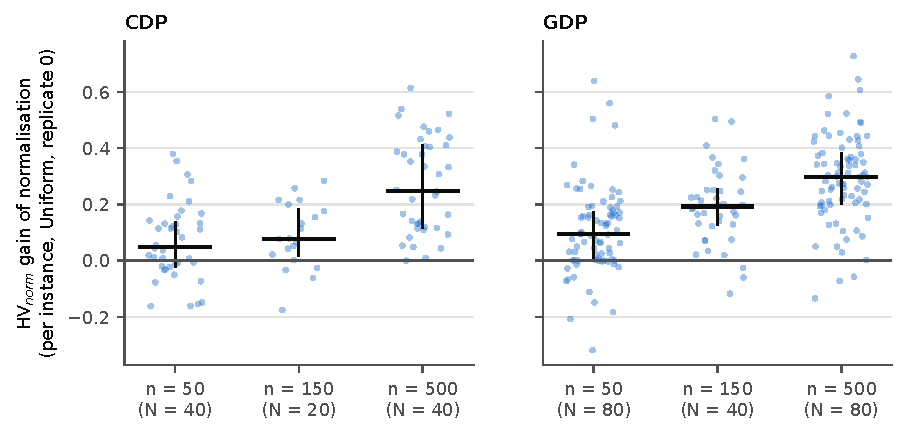
\includegraphics[width=\linewidth]{figures/fig1_normalisation_gain_vs_n.pdf}
\caption{Per-instance gain in $\mathrm{HV}_{\mathrm{norm}}$ from normalising the objectives (MOEA/D-Uniform, replicate 0; reference front fixed). Medians: CDP +0.05 (n = 50), +0.08 (n = 150), +0.25 (n = 500); GDP +0.09, +0.19, +0.30. The fraction of instances that improve rises from 0.65--0.78 at n = 50 to 0.96--1.00 at n = 500. Horizontal bars: medians; vertical bars: inter-quartile ranges.}\label{fig:1}
\end{figure}

\subsection{MOEA/D variants versus classical baselines (RQ1)}\label{sec:moea_d_variants_versus_class}

\begin{table}[t]
\centering
\small
\setlength{\tabcolsep}{4pt}
\caption{Average ranks ($\mathrm{HV}_{\mathrm{norm}}$, lower is better), normalised regime, mean over 3 replicates per instance; baselines with the fixed budgets of Appendix A and no tuning (tuned baselines: Tables 13 and 14)}\label{tab:1}
\begin{tabular}{lccc}
\toprule
Method & CDP (N=100) & GDP (N=200) & MDP (N=143) \\
\midrule
MOEA/D-GTS-HV & 3.61 & 3.25 & 4.20 \\
MOEA/D-Uniform & 3.62 & 3.53 & 4.50 \\
MOEA/D-UCB-HV & 3.78 & 3.65 & 4.25 \\
MOEA/D-GTS-Scal & 3.59 & 3.54 & 4.76 \\
MOEA/D-TS-HV & 4.01 & 3.71 & 5.01 \\
MOEA/D-TS-Scal & 5.10 & 5.25 & 5.31 \\
MOEA/D-UCB-Scal & 5.31 & 6.04 & 5.71 \\
GRASP-PR & 7.76 & 8.90 & 8.59 \\
GRASP-MO & 8.22 & 9.27 & 8.53 \\
VNS-Tcheb. & 11.48 & 10.79 & 7.39 \\
NSGA-II & 10.52 & 9.39 & 10.59 \\
VNS-Pareto & 11.00 & 10.67 & 9.16 \\
\emph{Friedman $\chi$$^{2}$ (p)} & 829.6 (8.4e-171) & 1593.3 (0.0e+00) & 642.9 (9.1e-131) \\
\emph{Nemenyi CD ($\alpha$=0.05)} & 1.67 & 1.18 & 1.39 \\
\emph{Significant pairs, Wilcoxon--Holm / Nemenyi (of 66)} & 55 / 44 & 53 / 51 & 51 / 42 \\
\bottomrule
\end{tabular}
\end{table}

\begin{itemize}
\item \textbf{CDP} top group (not distinguishable from the best, Wilcoxon--Holm): MOEA/D-GTS-Scal, MOEA/D-UCB-HV, MOEA/D-TS-HV, MOEA/D-GTS-HV, MOEA/D-Uniform.
\item \textbf{GDP} top group (not distinguishable from the best, Wilcoxon--Holm): MOEA/D-GTS-HV, MOEA/D-UCB-HV, MOEA/D-TS-HV, MOEA/D-GTS-Scal, MOEA/D-Uniform.
\item \textbf{MDP} top group (not distinguishable from the best, Wilcoxon--Holm): MOEA/D-GTS-HV, MOEA/D-UCB-HV, MOEA/D-GTS-Scal, MOEA/D-Uniform.
\end{itemize}

Table 1 gives the average ranks on the full catalogues (three replicates per instance). The Friedman test rejects equality in every problem, and 51--55 of the 66 pairs differ significantly under Wilcoxon--Holm (critical-difference diagrams in Figure 2). In all three problems the same picture holds: a top group of four or five MOEA/D configurations that cannot be told apart, followed by GRASP-PR/GRASP-MO, with NSGA-II and the VNS variants at the bottom. These baselines are the ones of the main experiment --- fixed budgets, no tuning --- and Section 6.12 repeats the comparison with tuned baselines, where the picture changes on the MDP. The gap between the worst member of the top group and the best baseline exceeds the critical difference in every problem (CDP: 4.01 versus 7.76, CD 1.67; GDP: 3.71 versus 8.90, CD 1.18; MDP: 4.76 versus 7.39, CD 1.39).

Two features differ between problems. On the MDP the baselines are closer: VNS-Tchebycheff ranks 7.39, ahead of the GRASP variants (8.5--8.6), whereas on CDP it ranks 11.5; on GDP NSGA-II (9.39) is on a par with the GRASP variants (8.90 and 9.27). In all three problems the GRASP variants fall 4--6 ranks behind the best-ranked configuration. Table 2 shows the same ordering in mean $\mathrm{HV}_{\mathrm{norm}}$, and the replicate noise: the coefficient of variation of $\mathrm{HV}_{\mathrm{norm}}$ across replicates is 8--15\% for MOEA/D, 14--21\% for GRASP and 18--30\% for NSGA-II and VNS-Pareto, so a single replicate per instance, as in our earlier catalogue, cannot support the finer rank differences.

\begin{table}[t]
\centering
\footnotesize
\setlength{\tabcolsep}{4pt}
\caption{Mean $\mathrm{HV}_{\mathrm{norm}}$ and between-replicate coefficient of variation (CV), full catalogue}\label{tab:2}
\begin{tabular}{lcccccc}
\toprule
Method & CDP $\mathrm{HV}_{\mathrm{norm}}$ & CDP CV & GDP $\mathrm{HV}_{\mathrm{norm}}$ & GDP CV & MDP $\mathrm{HV}_{\mathrm{norm}}$ & MDP CV \\
\midrule
MOEA/D-GTS-HV & 0.715 & 9\% & 0.737 & 13\% & 0.878 & 8\% \\
MOEA/D-Uniform & 0.714 & 10\% & 0.730 & 12\% & 0.871 & 8\% \\
MOEA/D-UCB-HV & 0.711 & 9\% & 0.721 & 15\% & 0.872 & 9\% \\
MOEA/D-GTS-Scal & 0.716 & 8\% & 0.726 & 12\% & 0.866 & 9\% \\
MOEA/D-TS-HV & 0.704 & 10\% & 0.721 & 13\% & 0.863 & 8\% \\
MOEA/D-TS-Scal & 0.688 & 10\% & 0.676 & 14\% & 0.849 & 10\% \\
MOEA/D-UCB-Scal & 0.684 & 9\% & 0.648 & 12\% & 0.838 & 10\% \\
GRASP-PR & 0.533 & 19\% & 0.345 & 14\% & 0.590 & 19\% \\
GRASP-MO & 0.518 & 15\% & 0.334 & 15\% & 0.583 & 21\% \\
VNS-Tcheb. & 0.223 & 14\% & 0.258 & 16\% & 0.621 & 11\% \\
NSGA-II & 0.275 & 22\% & 0.381 & 18\% & 0.431 & 29\% \\
VNS-Pareto & 0.234 & 21\% & 0.278 & 23\% & 0.535 & 30\% \\
\bottomrule
\end{tabular}
\end{table}

\begin{table}[t]
\centering
\footnotesize
\setlength{\tabcolsep}{4pt}
\caption{Ranks by instance-size regime (CDP/GDP; $\mathrm{HV}_{\mathrm{norm}}$)}\label{tab:3}
\begin{tabular}{lcccc}
\toprule
Method & CDP n$\leq$150 (N=60, 5 rep.) & CDP n=500 (N=40, 3 rep.) & GDP n$\leq$150 (N=120, 5 rep.) & GDP n=500 (N=80, 3 rep.) \\
\midrule
MOEA/D-GTS-HV & 3.87 & 3.60 & 3.62 & 2.89 \\
MOEA/D-Uniform & 3.45 & 3.58 & 3.42 & 3.75 \\
MOEA/D-UCB-HV & 3.58 & 3.80 & 3.41 & 3.46 \\
MOEA/D-GTS-Scal & 3.77 & 3.38 & 3.55 & 3.52 \\
MOEA/D-TS-HV & 3.98 & 4.03 & 3.76 & 3.54 \\
MOEA/D-TS-Scal & 5.02 & 4.88 & 5.49 & 5.19 \\
MOEA/D-UCB-Scal & 5.63 & 4.75 & 6.04 & 5.67 \\
GRASP-PR & 7.35 & 8.47 & 8.84 & 9.06 \\
GRASP-MO & 8.35 & 8.53 & 9.22 & 9.46 \\
VNS-Tcheb. & 11.13 & 11.95 & 10.70 & 10.97 \\
NSGA-II & 10.68 & 10.30 & 9.36 & 9.65 \\
VNS-Pareto & 11.18 & 10.75 & 10.59 & 10.82 \\
\bottomrule
\end{tabular}
\end{table}

\begin{figure}[t]
\centering
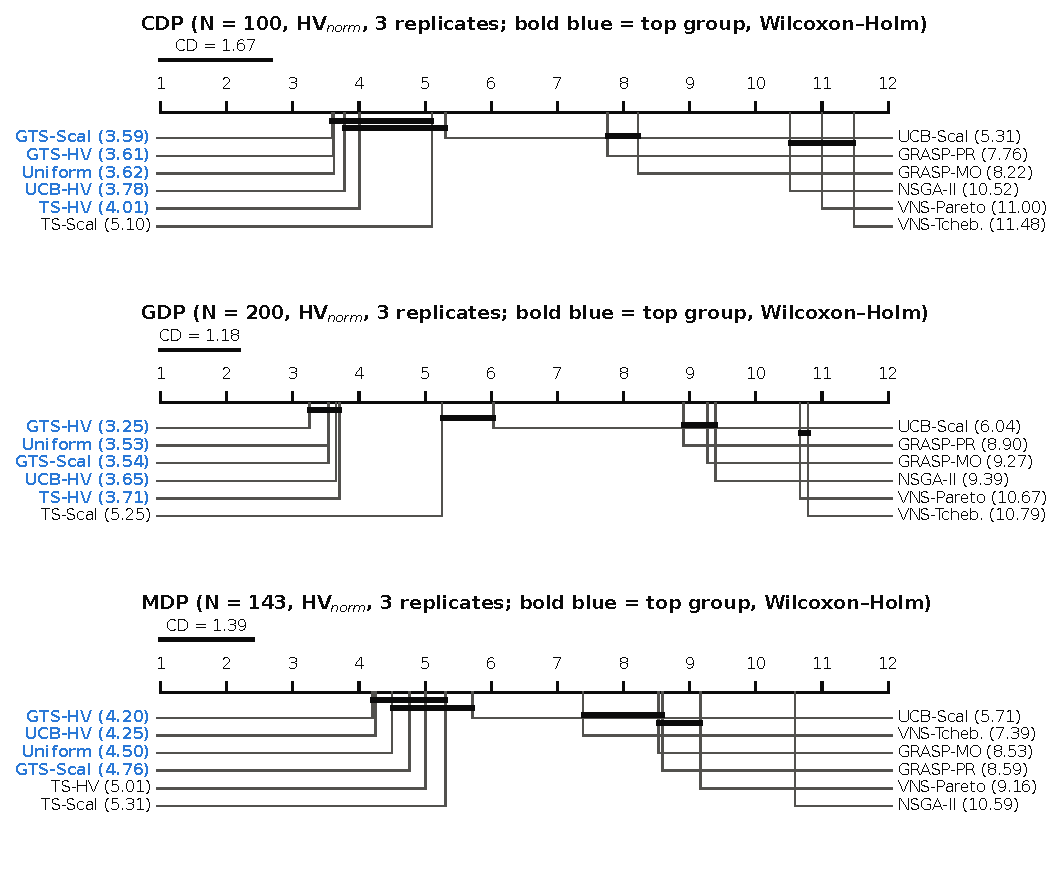
\includegraphics[width=\linewidth]{figures/fig4_cd_diagrams.pdf}
\caption{Critical-difference diagrams (Nemenyi, $\alpha$ = 0.05) of the twelve methods on the full catalogues: $\mathrm{HV}_{\mathrm{norm}}$, mean of three replicates per instance. Methods joined by a bar are not separated by the Nemenyi test; bold blue marks the top group under the Wilcoxon--Holm criterion, which is the primary criterion of this study.}\label{fig:2}
\end{figure}

Table 3 splits CDP and GDP by size. Rankings are stable between n $\leq$ 150 and n = 500 for the MOEA/D family; GRASP-PR and GRASP-MO lose ground as n grows (CDP: GRASP-PR 7.35 $\rightarrow$ 8.47; GDP: 8.84 $\rightarrow$ 9.06 and GRASP-MO 9.22 $\rightarrow$ 9.46), while NSGA-II is steady.

\emph{By family.} Supplement S2 breaks the average ranks down by instance family (descriptive only: 4--50 instances per MDP family, 20 per CDP group and 40 per GDP group). In the CDP and GDP the best baseline never ranks better than 6.25 (CDP, SOM-a) or 7.64 (GDP, SOM-a), i.e. it trails the best MOEA/D variant by 2.5 to 5.4 ranks (CDP) and 3.9 to 6.3 ranks (GDP) depending on family and size, the smallest gaps being on SOM-a. The MDP is where baselines come closest: VNS-Tchebycheff is the best baseline on SOM-a, SOM-b, MDG-b and MDG-a, and on MDG-a (ten instances) it is the best method overall (rank 3.80 against 4.70 for the best MOEA/D variant); on the sensor, facility and team application instances, on MGPO and on GKD-c the best baseline trails by 5.5--6.4 ranks, and on the portfolio instances GRASP-PR is within 1.4 ranks of the best MOEA/D variant (6.12 versus 4.75).

\subsection{Adaptive selection does not beat uniform selection on average (RQ2)}\label{sec:adaptive_selection_does_not_}

\begin{table}[t]
\centering
\small
\setlength{\tabcolsep}{4pt}
\caption{Each adaptive-selection variant against uniform operator selection (paired over instances; Wilcoxon--Holm over the six comparisons; $\hat{A}_{12}$ = P(variant better than uniform))}\label{tab:4}
\begin{tabular}{lccc}
\toprule
Variant & CDP: $\Delta$$\mathrm{HV}_{\mathrm{norm}}$, $\hat{A}_{12}$, p\_Holm & GDP: $\Delta$$\mathrm{HV}_{\mathrm{norm}}$, $\hat{A}_{12}$, p\_Holm & MDP: $\Delta$$\mathrm{HV}_{\mathrm{norm}}$, $\hat{A}_{12}$, p\_Holm \\
\midrule
MOEA/D-UCB-HV & $-$0.0035, 0.49, 1.0000 & $-$0.0092, 0.49, 1.0000 & +0.0009, 0.49, 1.0000 \\
MOEA/D-TS-HV & $-$0.0104, 0.48, 0.2951 & $-$0.0088, 0.49, 1.0000 & $-$0.0080, 0.48, 0.6393 \\
MOEA/D-GTS-HV & +0.0014, 0.50, 1.0000 & +0.0069, 0.51, 0.9342 & +0.0068, 0.51, 0.6393 \\
MOEA/D-UCB-Scal & $-$0.0306, 0.39, 0.0000 $^{*}$ & $-$0.0815, 0.32, 0.0000 $^{*}$ & $-$0.0337, 0.43, 0.0005 $^{*}$ \\
MOEA/D-TS-Scal & $-$0.0264, 0.39, 0.0001 $^{*}$ & $-$0.0540, 0.37, 0.0000 $^{*}$ & $-$0.0221, 0.44, 0.0009 $^{*}$ \\
MOEA/D-GTS-Scal & +0.0021, 0.52, 1.0000 & $-$0.0037, 0.50, 1.0000 & $-$0.0053, 0.48, 1.0000 \\
\bottomrule
\end{tabular}
\end{table}

(* = significantly \emph{worse} than uniform selection at 0.05 after Holm correction; no variant is significantly better in any problem.)

Table 4 compares each adaptive variant with uniform selection, paired over instances. No variant is significantly better than uniform selection in any of the three problems (largest $\hat{A}_{12}$ is 0.52). Two variants are significantly \emph{worse}, in all three problems: the scalar-reward bandits (UCB-Scal and TS-Scal). The ordering of the HV-reward variants among themselves is within replicate noise. The effect size of the loss for scalar-reward selectors is non-trivial ($\Delta$$\mathrm{HV}_{\mathrm{norm}}$ up to $-$0.08 on GDP, $\hat{A}_{12}$ = 0.32). These averages pool instances of all sizes; Section 6.11 shows that the verdict for the HV-reward selectors depends on instance size, on the tightness of the cost budget and on the generation budget.

\emph{Why.} Direct inspection of operator-selection frequencies (CDP, n = 50, full runs) explains the pattern. Under HV reward the bandits' reward is zero for every operator after roughly the first 20 generations because the population saturates the small front, so UCB1 and Thompson sampling degenerate to near-uniform selection (selection fractions 0.11--0.17 per operator even in the second half of the run) --- the HV-reward selectors \emph{are} uniform selection plus overhead. Under scalar reward the selectors do learn, but what they learn is myopic: they converge to MaxMinSwap and BiObjBestSwap (Figure 3: in the normalised CDP runs MaxMinSwap takes 0.51 of the selections of both UCB-Scal and TS-Scal and BiObjBestSwap 0.24 and 0.21; 0.66 for UCB-Scal in the raw regime), the operators that give the largest immediate Tchebycheff gain, and thereby lose the complementarity of the pool (Section 6.5). In the raw-objective regime the absolute-valued rewards also dwarf the exploration term of UCB1, which assumes rewards in [0,1]. The designs in Section 6.4 target these two failure modes and do not rescue the selectors. The Gaussian sampler with scalar reward (GTS-Scal) stays at 0.12--0.13 per operator, i.e. it is effectively uniform, which is why it ties with uniform selection.

\begin{figure}[t]
\centering
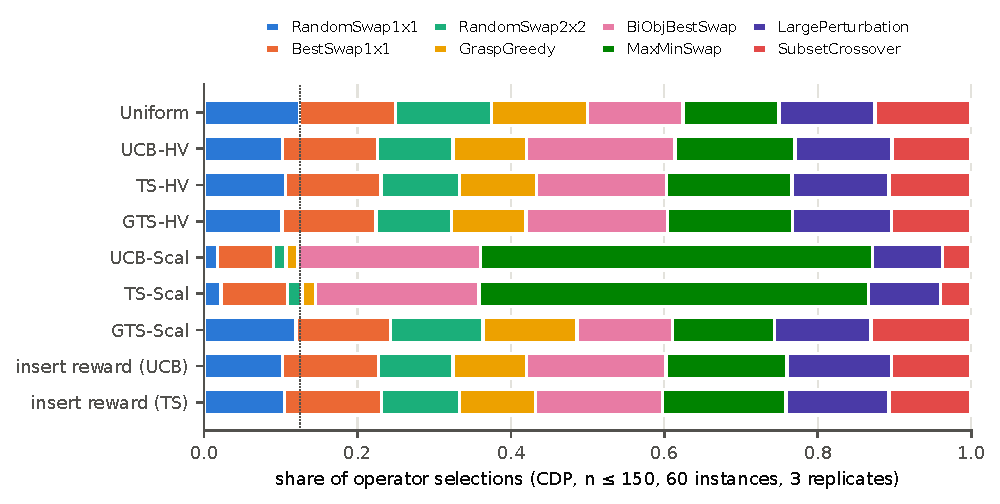
\includegraphics[width=\linewidth]{figures/fig2_operator_selection_shares.pdf}
\caption{Share of operator selections per selector and reward (CDP, n $\leq$ 150, 60 instances $\times$ 3 replicates, normalised regime; the dotted line marks 1/8). The HV-reward and insert-reward selectors stay within 0.09--0.20 per operator, and the scalar-reward UCB1 and Thompson sampling concentrate on MaxMinSwap and BiObjBestSwap.}\label{fig:3}
\end{figure}

\subsection{Attempts to repair adaptive selection}\label{sec:attempts_to_repair_adaptive_}

Since neither the HV reward nor the scalar reward gives a bandit much to learn from (Section 6.3), we tried five further families of designs on the 60 CDP and the 120 GDP instances with n $\leq$ 150 (three replicates; two relative-scalar variants of the first family on the CDP only), each against uniform selection on the same instances: (a) other reward signals --- an \emph{insert} reward (1 if the child enters the non-dominated archive) and the relative Tchebycheff improvement, each with cost-aware scaling or with a 50/50 exploration floor; (b) the dynamic Thompson sampling of \citet{sun2020} implemented exactly as published (Beta posteriors, binary \emph{replace} reward, decay threshold C $\in$ \{30, 100, 300\}); (c) contextual selection, with one bandit per third of the weight range and/or of the run; (d) a hyper-parameter sweep of the exploration constant and the window length of the UCB1 and Thompson selectors (17 settings); and (e) FRRMAB of \citet{li2014}, the MOEA/D selector with rank-based credit and a decaying bandit, with the published parameters and four others. We also doubled and quadrupled the generations, giving the selector and uniform selection the same budget. Table 5 summarises the outcome and Supplement S1 gives the details.

\begin{table}[t]
\centering
\footnotesize
\setlength{\tabcolsep}{4pt}
\caption{Attempts to repair adaptive selection, by family of variants (n $\leq$ 150, three replicates, each variant against uniform selection on the same instances; Wilcoxon p adjusted by Holm within the family): range of the difference in $\mathrm{HV}_{\mathrm{norm}}$ to uniform selection, and number of variants significantly better / worse (p < 0.05)}\label{tab:5}
\begin{tabular}{lccccc}
\toprule
Family & Variants & CDP (60 instances): difference & better / worse & GDP (120 instances): difference & better / worse \\
\midrule
Other rewards, cost-aware scaling, exploration floor & 8 & $-$0.024 to +0.003 & 0 / 1 & $-$0.017 to $-$0.007 & 0 / 0 \\
Faithful DYTS and the \texttt{replace} reward & 7 & $-$0.031 to $-$0.002 & 0 / 1 & $-$0.068 to $-$0.011 & 0 / 4 \\
Contextual selection (by weight and/or phase) & 7 & $-$0.012 to $-$0.001 & 0 / 0 & $-$0.015 to $-$0.009 & 0 / 0 \\
Hyper-parameter sweep (c, window) & 17 & $-$0.039 to +0.006 & 0 / 4 & $-$0.086 to +0.002 & 0 / 5 \\
FRRMAB \citep{li2014} & 5 & $-$0.011 to +0.006 & 0 / 0 & $-$0.017 to $-$0.007 & 0 / 1 \\
More generations ($\times$2, $\times$4), same budget for selector and uniform & 4 & $-$0.008 to +0.004 & 0 / 0 & $-$0.002 to +0.003 & 0 / 0 \\
\bottomrule
\end{tabular}
\end{table}

No variant is significantly better than uniform selection, in any family and in either problem (the largest $\hat{A}_{12}$ is 0.52), and between none and five variants per family are significantly worse --- those with a scalar or relative-scalar reward, which concentrate on MaxMinSwap and BiObjBestSwap and lose the complementarity of the pool, and on the GDP the published DYTS. Three observations matter for the argument. With the insert reward the selectors spread their selections moderately (0.10--0.18 per operator on the CDP), as with the HV reward, because the reward is zero for most children once the front is crowded. Cost-aware scaling did not make the search faster (median run time 2.70 s against 2.65 s without it on the CDP; 7.45 s against 7.71 s on the GDP). FRRMAB with its published parameters is effectively round-robin (0.124--0.127 of the selections per operator on the CDP): its credits are in [0, 1] and the scaling factor C = 5 makes the exploration term dominate; the published DYTS stays moderately spread (0.06--0.26 per operator on the CDP). Their equality with uniform selection is therefore explained by near-uniform behaviour, not by a badly tuned bandit. Two independent runs of uniform selection differ by +0.006 in $\mathrm{HV}_{\mathrm{norm}}$ ($\hat{A}_{12}$ 0.52, p = 0.23), which calibrates the noise: differences of that size between equivalent methods mean nothing. More generations help uniform selection (CDP +0.022 at $\times$2 and +0.036 at $\times$4; GDP +0.015 and +0.045; $p_{\mathrm{Holm}}$ < 0.01), but at the same budget no selector differs significantly from it. We conclude that on instances of this size no reward signal and no selector we tried identifies a state-independent best operator.

\subsection{The pool carries the performance (RQ4)}\label{sec:the_pool_carries_the_perform}

\emph{Single operators and leave-one-out.} We ran MOEA/D with uniform selection, normalised objectives and three replicates (CDP: 60 instances, GDP: 120; n $\leq$ 150) with one fixed operator and with the pool minus one operator, and compared each of the 16 variants with the full pool (Table 6; Holm over the 16 comparisons). Every operator alone is significantly worse than the pool ($p_{\mathrm{Holm}}$ < 0.01 in all 16 comparisons). The best single operator is RandomSwap1$\times$1 ($-$0.046 on the CDP, $-$0.036 on the GDP); the greedy and recombination operators are worst (GraspGreedy $-$0.29 and $-$0.41, BestSwap1$\times$1 $-$0.21 and $-$0.30, SubsetCrossover $-$0.20 and $-$0.40, MaxMinSwap $-$0.11 and $-$0.32). The myopic operators are poor alone and useful in the mix. Removing one operator from the pool hurts for only some of them. MaxMinSwap is indispensable in both problems ($-$0.036 on the CDP, p = 0.001; $-$0.039 on the GDP, p < 0.0001); on the GDP SubsetCrossover ($-$0.028, p = 0.0001) and RandomSwap2$\times$2 ($-$0.027, p = 0.003) also matter; and the other operators can be removed one at a time without a significant loss (the largest non-significant losses are $-$0.019 on the CDP, for SubsetCrossover, and $-$0.020 on the GDP, for LargePerturbation).

\begin{table}[t]
\centering
\footnotesize
\setlength{\tabcolsep}{4pt}
\caption{Operator ablation (n $\leq$ 150, three replicates): $\mathrm{HV}_{\mathrm{norm}}$ of MOEA/D with one operator only, and with the pool minus one operator, minus the $\mathrm{HV}_{\mathrm{norm}}$ of the full pool with uniform selection (Wilcoxon p adjusted by Holm over the 16 comparisons)}\label{tab:6}
\begin{tabular}{lcccc}
\toprule
Operator & CDP, only this operator & CDP, pool without it & GDP, only this operator & GDP, pool without it \\
\midrule
RandomSwap1$\times$1 & $-$0.046 (0.0086) & +0.003 (1) & $-$0.036 (0.0025) & $-$0.014 (0.064) \\
BestSwap1$\times$1 & $-$0.213 (2.6e$-$10) & +0.004 (1) & $-$0.302 (3.9e$-$20) & $-$0.006 (1) \\
RandomSwap2$\times$2 & $-$0.096 (9.7e$-$05) & $-$0.013 (0.75) & $-$0.074 (3.3e$-$08) & $-$0.027 (0.0025) \\
GraspGreedy & $-$0.286 (2.6e$-$10) & $-$0.008 (1) & $-$0.407 (3.3e$-$20) & $-$0.004 (1) \\
BiObjBestSwap & $-$0.082 (1.3e$-$09) & $-$0.003 (1) & $-$0.182 (1.1e$-$18) & $-$0.014 (0.52) \\
MaxMinSwap & $-$0.115 (2.4e$-$08) & $-$0.036 (0.001) & $-$0.321 (2.5e$-$17) & $-$0.039 (7.9e$-$06) \\
LargePerturbation & $-$0.154 (2.6e$-$10) & $-$0.007 (1) & $-$0.169 (4.1e$-$16) & $-$0.020 (0.27) \\
SubsetCrossover & $-$0.198 (2.6e$-$10) & $-$0.019 (0.23) & $-$0.402 (6e$-$20) & $-$0.028 (7.4e$-$05) \\
Full pool, uniform selection ($\mathrm{HV}_{\mathrm{norm}}$) & 0.711 &  & 0.771 &  \\
\bottomrule
\end{tabular}
\end{table}

\emph{Lean pools.} Dropping BiObjBestSwap, BestSwap1$\times$1 and GraspGreedy in combination (pools of seven, six and five operators; CDP, 60 instances, three replicates) leaves quality statistically equal to the full pool ($\Delta$$\mathrm{HV}_{\mathrm{norm}}$ between $-$0.008 and +0.010, $\hat{A}_{12}$ 0.44--0.52, all $p_{\mathrm{Holm}}$ = 1). Pruning saves little time: after vectorising the swap evaluation, BiObjBestSwap is no longer the dominant cost (the pool without it takes 106\% of the time of the full pool) and only dropping GraspGreedy saves 14--18\%. We keep the full pool: it is robust to pruning of the costly or redundant operators but not of MaxMinSwap.

\emph{A pool with harmful operators.} A natural objection to the finding that uniform selection suffices is that the pool is well curated, and that adaptive selection would earn its keep if some operators were useless. We added three deliberately bad operators to the eight --- a random restart (the solution is replaced by a random feasible one), a replacement of half of the elements at random, and a no-operation --- and repeated the experiment on the same instances, with uniform selection and with seven selectors (11 operators; Table 7). Uniform selection is not hurt: it gains +0.018 over the clean pool on the CDP (p = 0.084) and +0.002 on the GDP (p = 0.54), although 27\% of its effort now goes to the three new operators; the reason is that a child replaces a neighbour only if it is not worse, so a useless operator wastes effort but cannot damage the population, and the cost of the wasted effort is below the noise at the standard budget (doubling the generations gives +0.022; Section 6.4). No selector improves on uniform selection in the extended pool; UCB1 with the scalar reward is significantly worse on both problems ($-$0.038 and $-$0.071) and the published DYTS on the GDP ($-$0.024; p = 0.002). The selectors that learn something avoid the new operators only mildly (UCB1-HV: 0.07 of the selections for each of them against 0.09 under uniform selection), because the reward that would single them out is zero for almost every operator late in the run.

\begin{table}[t]
\centering
\small
\setlength{\tabcolsep}{4pt}
\caption{Pool with three harmful operators (random restart, half replacement, no-operation; 11 operators; n $\leq$ 150, three replicates): difference in $\mathrm{HV}_{\mathrm{norm}}$ of each selector to uniform selection in the same extended pool, and, in the first row, of uniform selection in the extended pool to uniform selection in the clean pool of eight (Holm-adjusted Wilcoxon p in brackets; an asterisk marks p < 0.05)}\label{tab:7}
\begin{tabular}{lcc}
\toprule
Selector in the extended pool & CDP (60 instances) & GDP (120 instances) \\
\midrule
Uniform, extended pool vs uniform, clean pool & +0.0182 (0.084) & +0.0019 (0.54) \\
UCB1-HV & $-$0.0048 (1) & $-$0.0080 (1) \\
GTS-HV & $-$0.0124 (0.53) & $-$0.0012 (1) \\
UCB1-Scal & $-$0.0382 (0.00061)$^{*}$ & $-$0.0708 (4.4e$-$11)$^{*}$ \\
GTS-Scal & $-$0.0072 (1) & $-$0.0053 (0.34) \\
UCB1, insert reward & $-$0.0165 (0.83) & $-$0.0043 (1) \\
DYTS (published), replace reward & $-$0.0134 (0.3) & $-$0.0236 (0.0017)$^{*}$ \\
FRRMAB & $-$0.0105 (1) & $-$0.0109 (0.34) \\
\bottomrule
\end{tabular}
\end{table}

\emph{Initialisation.} The weight-guided GRASP initialisation ($\alpha$ = 0.3) is not essential: a purely greedy start ($\alpha$ = 0) is as good (CDP +0.009, p = 0.20; GDP $-$0.006, p = 0.51), and a random start ($\alpha$ = 1) costs nothing on the CDP ($-$0.002, p = 0.60) but loses 0.051 of $\mathrm{HV}_{\mathrm{norm}}$ on the GDP (p = 0.032), where random solutions are further from feasibility.

\subsection{Covering the ends of the front: MaxMin anchoring and the literature (RQ3)}\label{sec:anchor_lit}

\emph{The gap.} With the unscaled scalarisation the MaxMin end of our fronts was far from published values: against the best published CDP value of each instance (see Section 5; 20 instances per family, both demand factors) the best MaxMin among all twelve methods (one replicate) was 10.6\% (SOM-a, n = 50), 5.2\% (GKD-b, n = 50), 9.0\% (GKD-b, n = 150), 12.8\% (GKD-c, n = 500) and 62.7\% (MDG-b, n = 500) below it; against the 80 published GDP solutions (n = 500) the ratios were 0.93--1.05 (GKD-c) and 0.45--0.50 (MDG-b). The published solutions are rarely dominated by our union front (0--7 of 20 per group) but lie in a region our front does not cover: high MaxMin, low MaxSum. Because the hypervolume is dominated by the knee of the front, this gap costs only 2.6--6.8\% of hypervolume on average --- the indicator hides it.

\emph{Normalisation helps but is not enough.} With normalised objectives (same comparison: best of the twelve methods, first replicate) the CDP ratios to the best published value rise from 0.894 to 0.936 (SOM-a), 0.948 to 0.972 (GKD-b, n = 50), 0.910 to 0.946 (GKD-b, n = 150), 0.872 to 0.905 (GKD-c) and 0.373 to 0.534 (MDG-b); on the GDP n = 500 pilot (five instances per family) the best MaxMin rises to 1.005 (GKD-c) and 0.69 (MDG-b) of the published value. In an earlier check against the Table 1 values of Gomez et al. (ten b02 instances per family), a trivial farthest-point constructive with 21 restarts reached $-$6.0\% (GKD-c) and $-$40.6\% (MDG-b), i.e. the MaxMin end of MOEA/D is only at the level of a simple heuristic.

\emph{Anchoring narrows the gap.} With the tabu anchoring step of Section 4.5 (Figure 4 and Table 8; uniform selection; the no-anchor reference is the same method without the step, on the same instances and replicates) the MaxMin end of the CDP fronts with n $\leq$ 150 moves to 1.000 of the best published value on SOM-a (20 of 20 instances reach it), 0.997 on GKD-b with n = 50 (14 of 20) and 0.984 with n = 150 (0 of 20), from 0.736, 0.935 and 0.929 (both demand factors pooled), and $\mathrm{HV}_{\mathrm{norm}}$ rises by +0.019 (better on 39 of 60 instances; Wilcoxon p = 0.015) at a cost of about two seconds per run. On the GDP (120 instances with n $\leq$ 150), which adds the budget constraint, the same step raises $\mathrm{HV}_{\mathrm{norm}}$ by +0.033 (better on 76 of 120; p = 0.0009) at a median extra cost of 0.9 s. At n = 500 (6,000 iterations $\times$ 3 restarts) the effect is larger. On the CDP $\mathrm{HV}_{\mathrm{norm}}$ rises by +0.073 (better on 37 of 40; p = 3$\cdot$10$^{-}$$^{1}$$^{0}$) and the MaxMin end moves from 0.865 to 0.972 of the best published value on GKD-c and from 0.473 to 0.697 on MDG-b (20 instances each; none reaches it); on the GDP $\mathrm{HV}_{\mathrm{norm}}$ rises by +0.052 (better on 61 of 80; p = 3$\cdot$10$^{-7}$) and the MaxMin end moves from 0.975 to 1.094 of the published value on GKD-c (at or above it on 30 of 40 instances) and from 0.592 to 0.917 on MDG-b (22 of 40). The step adds about 20 s to runs of 100--140 s. The published CDP values are the best of 40 runs of C++ solvers (the tabu search SBTS of \citet{lu2023}; for MDG-b also the VNS of \citet{mladenovic2022b} and the simulated annealing of \citet{rosati2024}); against the mean of the SBTS runs the anchored fronts reach 0.992 (GKD-c) and 0.911 (MDG-b) of the 10-s mean and 0.977 and 0.771 of the 300-s mean, and on MDG-b 0.705 of the best 300-s mean among the three solvers (Xeon 2.1 GHz and C++ against our Python implementation: indications, not an equal-time comparison). Adding the anchor point to \emph{every} method's front, or only to the MOEA/D variants, leaves the ranking between methods unchanged. Anchoring is therefore a coverage and competitiveness device, not a change to the comparison.

\begin{table}[t]
\centering
\footnotesize
\setlength{\tabcolsep}{4pt}
\caption{MaxMin anchoring (uniform selection, three replicates): $\mathrm{HV}_{\mathrm{norm}}$, paired difference to the same method without the step (uncorrected Wilcoxon p) and MaxMin end of the front relative to the best published value (CDP) or to the published 60-s VNS value (GDP), averaged over the instances of each family and both demand factors; median run time}\label{tab:8}
\begin{tabular}{lcccccc}
\toprule
Problem, size (N instances) & Families (order of the ratios) & Anchor & $\mathrm{HV}_{\mathrm{norm}}$ & Difference to none (p) & MaxMin end / published & Median time (s) \\
\midrule
CDP, n $\leq$ 150 (60) & SOM-a / GKD-b$_{50}$ / GKD-b$_{150}$ & none & 0.717 & -- & 0.736 / 0.935 / 0.929 & 3.5 \\
 &  & tabu & 0.736 & +0.019 (0.015) & 1.000 / 0.997 / 0.984 & 5.6 \\
 &  & SBTS & 0.729 & +0.012 (0.14) & 0.958 / 1.000 / 0.996 & 5.4 \\
 &  & combined & 0.737 & +0.020 (0.022) & 0.994 / 1.000 / 0.994 & 4.3 \\
CDP, n = 500 (40) & GKD-c / MDG-b & none & 0.719 & -- & 0.865 / 0.473 & 103.1 \\
 &  & tabu & 0.792 & +0.073 (3.1e-10) & 0.972 / 0.697 & 122.0 \\
 &  & SBTS & 0.753 & +0.034 (0.00094) & 0.994 / 0.895 & 230.9 \\
 &  & combined & 0.799 & +0.080 (5.6e-10) & 0.990 / 0.851 & 165.3 \\
GDP, n $\leq$ 150 (120) & -- & none & 0.756 & -- & -- & 3.9 \\
 &  & tabu & 0.790 & +0.033 (0.00091) & -- & 4.8 \\
 &  & SBTS & 0.787 & +0.030 (0.014) & -- & 4.2 \\
 &  & combined & 0.790 & +0.034 (0.00026) & -- & 4.0 \\
GDP, n = 500 (80) & GKD-c / MDG-b & none & 0.667 & -- & 0.975 / 0.592 & 116.9 \\
 &  & tabu & 0.720 & +0.052 (2.6e-07) & 1.094 / 0.917 & 137.9 \\
 &  & combined & 0.764 & +0.097 (7.7e-12) & 1.140 / 1.174 & 131.0 \\
\bottomrule
\end{tabular}
\end{table}

\begin{figure}[t]
\centering
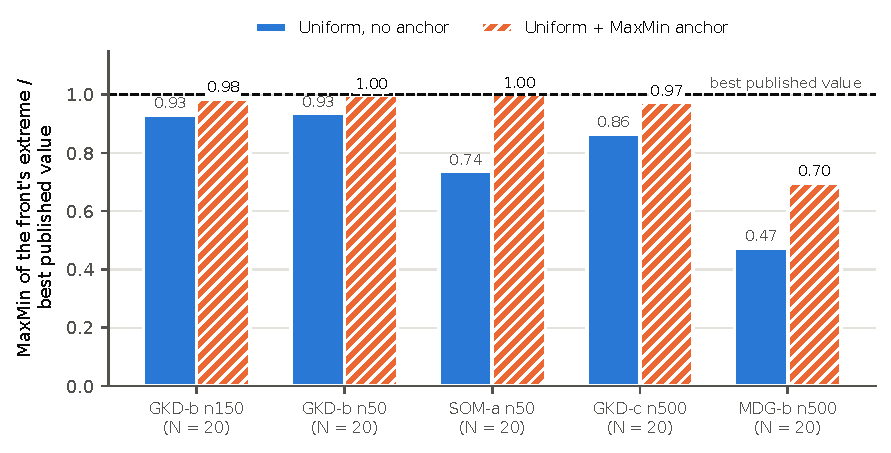
\includegraphics[width=\linewidth]{figures/fig3_extreme_maxmin_vs_published.pdf}
\caption{MaxMin of the front's extreme point relative to the best published CDP value (mean over instances, both demand factors, three replicates; Uniform selection, with and without the anchoring step). The dashed line is the best published value; budgets as in the text.}\label{fig:4}
\end{figure}

\emph{A stronger anchor.} The solution-based variant of Section 4.5 closes most of what remains on the CDP at n = 500 (40 instances, three replicates). With the SBTS-style search alone the MaxMin end reaches 0.994 (GKD-c) and 0.895 (MDG-b) of the best published value, against 0.972 and 0.697 for the tabu anchor, and 0.999 and 0.990 of the published 300-s SBTS mean (0.905 of the best 300-s mean among the three published solvers on MDG-b; eight of 20 GKD-c instances reach the best published value, none of MDG-b). The hypervolume tells a different story: the SBTS-style search alone is worse than the tabu anchor (0.753 against 0.792, p = 0.0002), because it does not add the intermediate points the tabu anchor contributes, whereas the combined anchor gives the best $\mathrm{HV}_{\mathrm{norm}}$ (0.799; +0.007 over the tabu anchor, p = 0.37) with MaxMin ends of 0.990 and 0.851. The cost is substantial at n = 500: median run times of 103 s without anchor, 122 s with the tabu anchor, 165 s with the combined anchor and 231 s with the SBTS-style search alone. For n $\leq$ 150 (60 CDP instances) the combined anchor reaches 0.994 (GKD-b, n = 150), 1.000 (GKD-b, n = 50) and 0.994 (SOM-a) of the best published value, with the same $\mathrm{HV}_{\mathrm{norm}}$ as the tabu anchor (difference +0.001, p = 0.88) and no additional cost to speak of. On the GDP the combined anchor is better than the tabu anchor where the budget binds hardest: at n = 500 (80 instances) $\mathrm{HV}_{\mathrm{norm}}$ is 0.764 against 0.720 (+0.045, p = 7$\cdot$10$^{-5}$) and the MaxMin end reaches 1.140 (GKD-c; 33 of 40 instances at or above the published value) and 1.174 (MDG-b; 31 of 40) of the value published for the benchmark's 60-s VNS, at a median run time of 131 s (117 s without anchor); for n $\leq$ 150 (120 instances) the two anchors are indistinguishable. Using GTS-HV instead of uniform selection with the combined anchor gives the same gains (CDP n $\leq$ 150: +0.018, p = 0.039; GDP n $\leq$ 150: +0.035, p < 0.0001; both against uniform selection without anchor). The remaining gap to the best published values is the MDG-b family of the CDP (0.85--0.90).

\subsection{Robustness of the comparison to the evaluation protocol}\label{sec:robustness_of_the_comparison}

\emph{Budget fairness: baselines at equal wall-clock time.} Generation- and iteration-based budgets favour methods that are cheap per step, so we repeated the comparison with equal wall-clock time (Table 9). For every (instance, replicate) the normalised MOEA/D-Uniform was run first in a worker process and its elapsed time T measured; NSGA-II, VNS-Pareto (without early stopping), VNS-Tchebycheff and the two GRASP variants were then run in the same process with a time limit of T (their initialisation time is not counted, which favours them). The sample is every instance with n $\leq$ 150 (CDP: 60; GDP: 120) and a subset of the n = 500 instances (CDP: 20, half with each demand factor; GDP: 40, half with the tightest and half with the loosest combination of demand and cost factors, 0.2/0.2 and 0.3/0.3), with three replicates. The median limits are 2.3 s and 67 s on CDP and 3.4 s and 92 s on GDP (the n $\leq$ 150 group mixes n = 50 and n = 150, so its limits are short). Extra time improves every baseline over its default budget (by +0.01 to +0.12 $\mathrm{HV}_{\mathrm{norm}}$) but, with one exception, does not close the gap: NSGA-II, the two VNS variants and, on GDP and at n = 500, GRASP-MO and GRASP-PR remain significantly behind MOEA/D-Uniform (Holm p < 10$^{-5}$ in all those cases). The exception is CDP with n $\leq$ 150, where GRASP-PR and GRASP-MO at equal time are statistically tied with MOEA/D-Uniform ($\mathrm{HV}_{\mathrm{norm}}$ 0.705 and 0.693 against 0.711; $\hat{A}_{12}$ 0.43 and 0.40; $p_{\mathrm{Holm}}$ = 0.61 and 0.29 over 60 instances). The superiority of MOEA/D over GRASP on CDP is therefore established at n = 500 but not for short runs on small instances. An earlier pilot in the raw regime with six CDP instances and budgets scaled to the recorded MOEA/D time gave the same picture for NSGA-II and VNS (ranks 10--12 of 12 before and after). Extra VNS budget helps little because the limit is the search design: three greedy neighbourhoods around archive members.

\begin{table}[t]
\centering
\scriptsize
\setlength{\tabcolsep}{4pt}
\caption{Baselines at equal wall-clock time (normalised regime, three replicates): mean $\mathrm{HV}_{\mathrm{norm}}$; in brackets, difference to MOEA/D-Uniform and Holm-adjusted Wilcoxon p (paired over instances)}\label{tab:9}
\resizebox{\linewidth}{!}{%
\begin{tabular}{lcccccc}
\toprule
Problem, size (N instances; time limit per run) & MOEA/D-Uniform & GRASP-PR & GRASP-MO & NSGA-II & VNS-Pareto & VNS-Tcheb. \\
\midrule
CDP n<=150 (N=60; 2 s) & 0.711 & 0.705 ($-$0.006; p=0.61) & 0.693 ($-$0.018; p=0.29) & 0.456 ($-$0.255; p=8.1e-11) & 0.351 ($-$0.360; p=8.1e-11) & 0.379 ($-$0.332; p=8.1e-11) \\
CDP n=500 (N=20; 67 s) & 0.721 & 0.430 ($-$0.291; p=9.5e-06) & 0.432 ($-$0.288; p=9.5e-06) & 0.285 ($-$0.435; p=9.5e-06) & 0.156 ($-$0.565; p=9.5e-06) & 0.161 ($-$0.559; p=9.5e-06) \\
GDP n<=150 (N=120; 3 s) & 0.771 & 0.489 ($-$0.282; p=2.4e-12) & 0.485 ($-$0.286; p=2.4e-12) & 0.559 ($-$0.213; p=5e-20) & 0.443 ($-$0.329; p=9.9e-21) & 0.436 ($-$0.336; p=9.9e-21) \\
GDP n=500 (N=40; 92 s) & 0.681 & 0.321 ($-$0.360; p=9.1e-12) & 0.299 ($-$0.382; p=9.1e-12) & 0.221 ($-$0.461; p=9.1e-12) & 0.154 ($-$0.528; p=9.1e-12) & 0.188 ($-$0.493; p=9.1e-12) \\
\bottomrule
\end{tabular}
}
\end{table}

\emph{Reference front.} Ranking with a front pooled over the methods compared, or with the fixed union reference, is practically identical (Kendall $\tau$ = 1.00 on GDP, 0.88 on CDP; differences confined to the top group).

\subsection{Robustness to the quality indicator}\label{sec:robustness_to_the_quality_in}

\begin{table}[t]
\centering
\scriptsize
\setlength{\tabcolsep}{4pt}
\caption{Robustness to the quality indicator (full catalogue): Kendall's $\tau$ between the average-rank vectors, and top group per indicator}\label{tab:10}
\begin{tabularx}{\linewidth}{lcccXXX}
\toprule
Problem & $\tau$($\mathrm{HV}_{\mathrm{norm}}$, IGD$^{+}$) & $\tau$($\mathrm{HV}_{\mathrm{norm}}$, $\varepsilon^{+}$) & $\tau$(IGD$^{+}$, $\varepsilon^{+}$) & Top group $\mathrm{HV}_{\mathrm{norm}}$ & Top group IGD$^{+}$ & Top group $\varepsilon^{+}$ \\
\midrule
CDP & 0.94 & 0.79 & 0.73 & MOEA/D-GTS-Scal, MOEA/D-UCB-HV, MOEA/D-TS-HV, MOEA/D-GTS-HV, MOEA/D-Uniform & MOEA/D-Uniform, MOEA/D-UCB-HV, MOEA/D-GTS-HV, MOEA/D-GTS-Scal & MOEA/D-UCB-HV, MOEA/D-TS-HV, MOEA/D-GTS-HV, MOEA/D-GTS-Scal, MOEA/D-Uniform \\
GDP & 1.00 & 0.97 & 0.97 & MOEA/D-GTS-HV, MOEA/D-UCB-HV, MOEA/D-TS-HV, MOEA/D-GTS-Scal, MOEA/D-Uniform & MOEA/D-GTS-HV, MOEA/D-UCB-HV, MOEA/D-TS-HV, MOEA/D-GTS-Scal, MOEA/D-Uniform & MOEA/D-GTS-HV, MOEA/D-UCB-HV, MOEA/D-TS-HV, MOEA/D-GTS-Scal, MOEA/D-Uniform \\
MDP & 0.91 & 0.85 & 0.88 & MOEA/D-GTS-HV, MOEA/D-UCB-HV, MOEA/D-GTS-Scal, MOEA/D-Uniform & MOEA/D-UCB-HV, MOEA/D-TS-HV, MOEA/D-GTS-HV, MOEA/D-GTS-Scal, MOEA/D-Uniform & MOEA/D-Uniform, MOEA/D-UCB-HV, MOEA/D-TS-HV, MOEA/D-GTS-HV, MOEA/D-GTS-Scal \\
\bottomrule
\end{tabularx}
\end{table}

$\mathrm{HV}_{\mathrm{norm}}$, IGD$^{+}$ and $\varepsilon$$^{+}$ produce closely related rankings (Kendall's $\tau$ between 0.73 and 1.00, Table 10). The top groups coincide up to the membership of marginal variants (TS-HV on the CDP, TS-Scal on the MDP), which enter or leave depending on the indicator. On the CDP data with n $\leq$ 150 and five replicates, $\varepsilon$$^{+}$ --- a worst-case measure sensitive to the ends of the front --- also admitted GRASP-PR into the top group; this does not occur on the full catalogue with three replicates. The conclusions that the MOEA/D family is ahead of the baselines and that no adaptive selector beats uniform selection do not depend on the indicator.

\subsection{Why GRASP behaves differently on CDP and GDP}\label{sec:why_grasp_behaves_differentl}

On the raw-objective catalogue, GRASP-MO/PR were tied with MOEA/D on CDP but fell to the middle tier on GDP, and NSGA-II moved in the opposite direction; with normalised objectives the GRASP variants are behind MOEA/D on both problems (Table 1), but the CDP/GDP contrast in how far behind persists (CDP: GRASP-PR 7.75; GDP: 8.91) and so does the contrast for NSGA-II (CDP 10.52; GDP 9.39). To test whether the GDP budget constraint explains it, we re-ran all twelve methods in the normalised regime with the budget relaxed to infinity (leaving only the capacity constraint) on the 120 GDP instances with n $\leq$ 150 and on twenty instances with n = 500 (ten with the tightest and ten with the loosest combination of demand and cost factors), three replicates each and the same seeds as the original runs, and compared the ranks of the twelve methods within each regime (each regime has its own reference front, because relaxed solutions may violate the original budget). Relaxing the budget improves GRASP-PR (average rank 8.93 $\rightarrow$ 7.57) and GRASP-MO (9.32 $\rightarrow$ 8.29) significantly (Wilcoxon on per-instance ranks, Holm p < 0.0001), worsens NSGA-II (9.20 $\rightarrow$ 10.29) and VNS-Pareto (10.55 $\rightarrow$ 11.56) significantly (p < 0.0001), and moves the MOEA/D variants by less than 0.8 ranks (UCB-Scal improves by 0.76, p = 0.010; none of the others is significant, the largest change being GTS-HV +0.58, p = 0.11). The budget constraint is therefore a major driver of how GRASP and NSGA-II compare with the MOEA/D family on GDP, but the reversal is partial: relaxed GRASP-PR (7.57) remains four ranks behind the best method (3.48; CD = 1.52). On the twenty n = 500 instances no change is significant (little power at N = 20; GRASP-PR 8.60 $\rightarrow$ 8.40, NSGA-II 9.55 $\rightarrow$ 9.75); the one notable movement is that GTS-HV loses 1.90 ranks when the cost budget is relaxed (2.65 $\rightarrow$ 4.55, $p_{\mathrm{Holm}}$ = 0.065), which fits the finding of Section 6.11 that its advantage over uniform selection is tied to the tight cost budget.

\subsection{Larger instances: a scalability sample}\label{sec:larger_instances_a_scalabili}

The main comparison stops at n = 500 (CDP, GDP) and n = 1,000 (MDP). To see whether the findings extend to larger instances we ran a small sample: three MDG-b instances with n = 2,000 (m = 200) and two MDG-c instances with n = 3,000 (m = 400), with three replicates and six methods (MOEA/D with uniform selection, with UCB1 and with the Gaussian sampler under the HV reward, NSGA-II, GRASP-PR and VNS-Tchebycheff), in the normalised regime and with the largest budget of Appendix A (100 weight vectors, 600 generations). Five instances support no inference; the results are descriptive, and the reference front of each instance is the union of the runs of this sample.

\begin{table}[t]
\centering
\footnotesize
\setlength{\tabcolsep}{4pt}
\caption{Scalability sample (MDP, normalised regime, three replicates; reference front per instance = union of all runs of the sample): $\mathrm{HV}_{\mathrm{norm}}$ per instance (mean of three replicates); last rows: median run time over instances and average front size}\label{tab:11}
\begin{tabular}{lcccccc}
\toprule
Instance & MOEA/D-Uniform & MOEA/D-UCB-HV & MOEA/D-GTS-HV & NSGA-II & GRASP-PR & VNS-Tcheb. \\
\midrule
MDG-b\_21\_n2000\_m200 & 0.697 & 0.880 & 0.858 & 0.052 & 0.274 & 0.008 \\
MDG-b\_31\_n2000\_m200 & 0.720 & 0.898 & 0.868 & 0.060 & 0.156 & 0.005 \\
MDG-b\_40\_n2000\_m200 & 0.688 & 0.787 & 0.803 & 0.061 & 0.103 & 0.011 \\
\emph{median time per run (s), all five instances} & 848 & 981 & 945 & 54 & 1438 & 30 \\
\emph{average front size, all five instances} & 45.7 & 56.7 & 53.7 & 6.1 & 6.7 & 3.0 \\
\bottomrule
\end{tabular}
\end{table}

\emph{MDG-c, n = 3000 (two instances): the front is a single point with MaxMin = 0 for every method in every run but one GRASP-PR replicate, so $\mathrm{HV}_{\mathrm{norm}}$ is not informative; best MaxSum found (mean of three replicates, in millions; mean over the two instances):}

\begin{center}
\footnotesize
\setlength{\tabcolsep}{4pt}
\begin{tabular}{lcccccc}
\toprule
 & MOEA/D-Uniform & MOEA/D-UCB-HV & MOEA/D-GTS-HV & NSGA-II & GRASP-PR & VNS-Tcheb. \\
\midrule
MaxSum ($\times$10$^{6}$) & 43.19 & 43.21 & 43.22 & 42.91 & 42.73 & 42.65 \\
\bottomrule
\end{tabular}
\end{center}

On MDG-b with n = 2,000 the baselines are far behind (Table 11), as at smaller sizes: NSGA-II reaches $\mathrm{HV}_{\mathrm{norm}}$ 0.05--0.06, GRASP-PR 0.10--0.27 and VNS-Tchebycheff at most 0.01, against 0.69--0.90 for MOEA/D. \textbf{The comparison among MOEA/D variants differs from Sections 6.3--6.5.} On all three instances the two HV-reward selectors beat uniform selection (0.88, 0.90 and 0.79 for UCB1 and 0.86, 0.87 and 0.80 for the Gaussian sampler, against 0.70, 0.72 and 0.69), and each is above the uniform replicate of the same index in eight of the nine (instance, replicate) cells. The gain comes from the MaxMin end of the front (mean best MaxMin 18.4 for UCB1 against 14.8 for uniform selection over the nine runs, with MaxSum unchanged within 0.2\%). The selectors behave unlike the near-uniform HV selectors of Section 6.3: they concentrate on BiObjBestSwap (0.32--0.39 of the selections) and MaxMinSwap (0.35--0.40) and give SubsetCrossover 0.07--0.15, which is what one would expect if the HV reward does not saturate because the search is far from converged --- 600 generations over 2,000 elements. Section 6.11 tests the explanation that adaptive selection helps when the search is far from convergence. Run times are about 850 s for uniform selection and 950--980 s for the two adaptive variants, 54 s for NSGA-II, 1,440 s for GRASP-PR and 30 s for VNS-Tchebycheff, on a shared laptop.

On MDG-c with n = 3,000 the bi-objective problem is degenerate: the integer distances include a few thousand exact zeros, almost every subset has MaxMin = 0, and the front of every method in every run is a single point with MaxMin = 0, except one GRASP-PR replicate that also found a point with MaxMin = 7 at 5\% lower MaxSum than its other point. $\mathrm{HV}_{\mathrm{norm}}$ is therefore not informative there, and the comparison reduces to MaxSum: the three MOEA/D variants reach 43.1--43.3 million (indistinguishable), NSGA-II about 0.7\% lower, GRASP-PR about 1.1\% lower and VNS-Tchebycheff about 1.3\% lower. The MaxMin anchor does not apply to the MDP (fixed cardinality), so the MaxMin end of the MDG-c front is not covered by any method.

\subsection{When adaptive selection helps: instance size, constraint tightness and budget}\label{sec:when_adaptive_selection_help}

The averages of Section 6.3 pool instances of all sizes. Splitting the per-instance difference between each HV-reward selector and uniform selection by size (Figure 5; fixed reference front, mean over three replicates, descriptive 95\% bootstrap intervals over instances) reveals a size effect.

\begin{figure}[t]
\centering
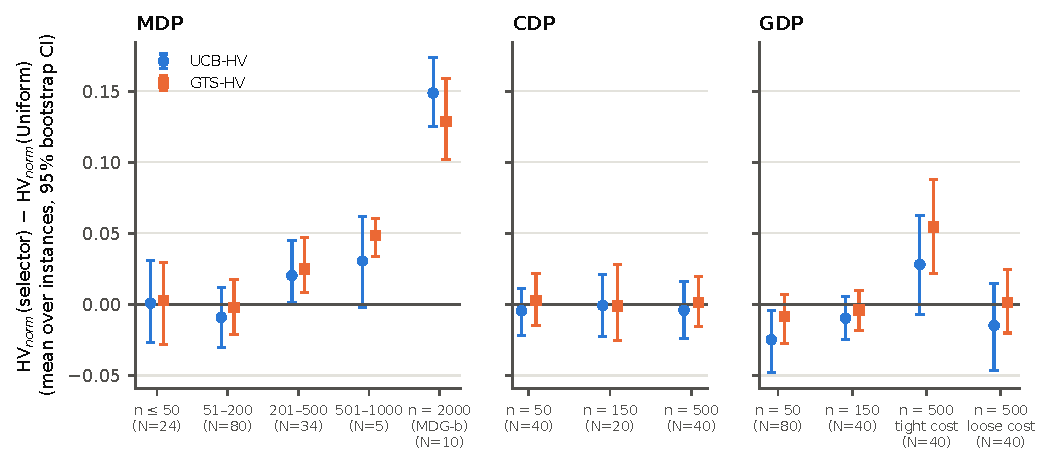
\includegraphics[width=\linewidth]{figures/fig5_adaptive_selection_vs_size.pdf}
\caption{Difference in $\mathrm{HV}_{\mathrm{norm}}$ between the HV-reward selectors and uniform selection, by problem and instance size (mean over instances of the mean over three replicates; bars: 95\% bootstrap intervals over instances; fixed reference fronts, except n = 2,000, whose reference is the union of the scalability and budget-regime runs). MDP: no difference up to 200 elements, a growing advantage beyond. GDP: advantage only with n = 500 and the tight cost budget. CDP: none.}\label{fig:5}
\end{figure}

In the MDP the difference is zero up to 200 elements (n $\leq$ 50: UCB-HV +0.001, GTS-HV +0.003, N = 24; 51--200: $-$0.009 and $-$0.002, N = 80), positive at 201--500 elements (+0.020 and +0.025, N = 34; Wilcoxon p = 0.075 and 0.009, uncorrected), larger at 501--1,000 (+0.031 and +0.049, N = 5, MGPO only) and largest at 2,000 (MDG-b, N = 10: +0.149 and +0.129). In the CDP it stays at zero up to n = 500 ($-$0.004 and +0.001, N = 40). In the GDP it is $\leq$ 0 up to n = 150 and positive at n = 500 only on the 40 instances with the tight cost budget (factor 0.2: +0.028 and +0.054, p = 0.075 and 0.0009 uncorrected), not on the 40 with the loose one (factor 0.3: $-$0.015 and +0.001). The p-values in this paragraph are uncorrected for the number of size groups and are exploratory; the experiment below is the confirmatory test.

\emph{Budget.} If the effect comes from searches that are far from convergence, it should grow as the generation budget shrinks. We changed the number of generations while holding the instances fixed (three replicates, the same seeds as the 1$\times$ runs): \textonequarter{}, \textonehalf{} and 1$\times$ the generations of Appendix A on the 40 CDP, the 40 tight-budget GDP and the 40 loose-budget GDP instances with n = 500, and 1$\times$ on ten MDG-b instances with n = 2,000 plus 4$\times$ on three of them (Table 12). On the tight-budget GDP the advantage of the HV-reward selectors is monotone in the budget: UCB-HV +0.059, +0.035 and +0.028 and GTS-HV +0.067, +0.059 and +0.054 at \textonequarter{}, \textonehalf{} and 1$\times$ (Holm p $\leq$ 0.024 for five of the six comparisons; IGD$^{+}$ gives the same ordering). On the loose-budget GDP and on the CDP there is no effect at any budget (the largest difference is +0.025, GTS-HV on the CDP at \textonequarter{}; no comparison is significant), although the selectors there concentrate on the same two operators as elsewhere (0.66--0.68 of the selections at \textonequarter{}): concentration alone does not pay. On MDG-b with n = 2,000 both selectors beat uniform selection on all ten instances at the standard budget ($p_{\mathrm{Holm}}$ = 0.004, the smallest value the test allows with ten instances; IGD$^{+}$: +0.057 and +0.050, ten of ten) and the advantage shrinks but does not vanish with four times the generations (three instances: UCB-HV +0.139 $\rightarrow$ +0.112, GTS-HV +0.129 $\rightarrow$ +0.084).

\begin{table}[t]
\centering
\footnotesize
\setlength{\tabcolsep}{4pt}
\caption{HV-reward adaptive selection against uniform selection at the same budget (instances with n = 500 or n = 2,000; three replicates; budget = fraction or multiple of the generations of Appendix A): $\mathrm{HV}_{\mathrm{norm}}$ of uniform selection, and difference to it (Holm-adjusted Wilcoxon p, paired over instances) for UCB1-HV and GTS-HV}\label{tab:13}
\begin{tabularx}{\linewidth}{lccccX}
\toprule
Setting (N instances) & Budget & Uniform & UCB-HV $-$ Uniform (p) & GTS-HV $-$ Uniform (p) & Share of BiObjBestSwap + MaxMinSwap: UCB-HV \\
\midrule
CDP n=500 (N=40) & x1/4 & 0.661 & +0.014 (0.675) & +0.025 (0.134) & 0.68 \\
CDP n=500 (N=40) & x1/2 & 0.695 & +0.003 (1) & +0.012 (1) & 0.58 \\
CDP n=500 (N=40) & x1 & 0.719 & $-$0.004 (1) & +0.001 (1) & 0.49 \\
GDP n=500, k02 (tight cost budget) (N=40) & x1/4 & 0.505 & +0.059 (0.000308) & +0.067 (2.96e-05) & 0.48 \\
GDP n=500, k02 (tight cost budget) (N=40) & x1/2 & 0.587 & +0.035 (0.024) & +0.059 (0.000191) & 0.44 \\
GDP n=500, k02 (tight cost budget) (N=40) & x1 & 0.644 & +0.028 (0.0747) & +0.054 (0.00267) & 0.39 \\
GDP n=500, k03 (N=40) & x1/4 & 0.622 & +0.005 (1) & +0.019 (1) & 0.68 \\
GDP n=500, k03 (N=40) & x1/2 & 0.659 & $-$0.006 (1) & +0.010 (1) & 0.58 \\
GDP n=500, k03 (N=40) & x1 & 0.691 & $-$0.015 (1) & +0.001 (1) & 0.50 \\
MDP MDG-b n=2000 (N=10) & x1 & 0.679 & +0.149 (0.00391) & +0.129 (0.00391) & 0.74 \\
MDG-b n = 2000, three instances (N=3) & x1 & 0.643 & +0.139 (n/a) & +0.129 (n/a) & 0.76 \\
MDG-b n = 2000, three instances (N=3) & x4 & 0.754 & +0.112 (n/a) & +0.084 (n/a) & 0.51 \\
\bottomrule
\end{tabularx}
\end{table}

\emph{Why the tight cost budget matters.} Our first hypothesis was that, with a tight budget, the repair step discards many children of the operators that ignore the cost, so that the success rates of the operators differ more than with a loose budget and there is more to learn. We tested it by re-running 540 standard-budget runs (ten instances in each of three groups at n = 500, and in three at n = 150; same seeds, identical fronts) with per-operator counters (Supplement S3). The first half of the hypothesis holds: on the tight-budget GDP 34\% of all children are infeasible before the repair at n = 500 (45\% at n = 150), against 0.3\% on the loose-budget GDP and 0.7\% on the CDP, and the six cost-blind operators produce between 34\% and 60\% infeasible children. The second half does not: BiObjBestSwap and MaxMinSwap insert 0.07--0.11 children per application into the archive and the other six at most 0.02 in every group, and the dispersion of the insertion rates across operators is not larger under the tight budget (standard deviation 0.037, against 0.035 on the loose GDP and 0.038 on the CDP). What differs is how far the search is from convergence at the standard budget: uniform selection gains 0.139 in $\mathrm{HV}_{\mathrm{norm}}$ when its budget grows from a quarter to the standard one on the tight GDP, against 0.068 on the loose GDP and 0.058 on the CDP (n = 500, 40 instances each). A plausible chain is therefore that the tight budget makes a third of the children need repair, progress per generation slows, the search is far from convergence at the standard budget, and moving effort from the six weak operators to the two productive ones pays --- which is what the HV-reward selectors do (0.57 of the selections of UCB-HV on the tight GDP, against 0.47 and 0.51). The evidence is at the level of the three instance groups: across instances within a group the advantage of the selectors is not correlated with the convergence slope (|$\rho$| $\leq$ 0.22, p $\geq$ 0.16) and across the 120 instances the correlation is weak ($\rho$ = +0.14, p = 0.13 for GTS-HV), so the mechanism is established for groups and open for individual instances.

\emph{Reading.} Adaptive selection with the HV reward gains where the search is short of convergence and the instance is either large (MDG-b with 2,000 elements) or has a tight constraint to repair (GDP with the 0.2 cost factor); it does not where the reward saturates early (CDP at the sizes tested, every problem below 200 elements) or where the constraint is loose. Budget scarcity explains the dose--response on the tight GDP and the shrinkage at n = 2,000 but not, by itself, the absence of an effect on the CDP with a quarter of the generations, nor on the loose GDP, whose convergence slopes are similar to the CDP's; the measured slope on the tight GDP is twice as large. The verdict of Section 6.3 stands for the regime in which the earlier benchmarks of this literature live (n $\leq$ 200) and for the CDP; it does not extend to large or tightly constrained instances.

\subsection{Tuned baselines and the trajectory methods of Colmenar et al. (RQ1)}\label{sec:tuned_baselines_and_the_traj}

The baselines of Sections 6.2 and 6.7 run with fixed budgets and without tuning, whereas Colmenar et al. tuned every method with irace. Section 4.7 describes the protocol that gives every method --- NSGA-II, SMS-EMOA, GRASP, a tabu search and a VNS in the style of Colmenar et al., and the uniform-pool MOEA/D --- a tuning of the same size on held-out instances; Tables 13 and 14 report six cells (CDP, GDP and MDP; n $\leq$ 150 and n = 500) with the wall-clock time of the default MOEA/D-Uniform on the same instance and replicate (initialisation included; the median measured time of every method was within 1\% of its limit) and, for part of the instances, five times that time.

\begin{table}[t]
\centering
\footnotesize
\setlength{\tabcolsep}{4pt}
\caption{Tuned baselines and the tabu search and VNS of Colmenar et al. against the default MOEA/D-Uniform (normalised regime; $\mathrm{HV}_{\mathrm{norm}}$ against the frozen reference, mean over held-out test instances and replicates; in brackets the paired difference to MOEA/D-Uniform with the default setting, an asterisk marks Holm-adjusted Wilcoxon p < 0.05; N = test instances). All methods run with the wall-clock time of the default MOEA/D-Uniform on the same instance and replicate (initialisation included); the last block gives five times that time (first replicate only)}\label{tab:14}
\begin{tabular}{lcccccc}
\toprule
Method & CDP n $\leq$ 150 & CDP n = 500 & GDP n $\leq$ 150 & GDP n = 500 & MDP n $\leq$ 150 & MDP n = 500 \\
\midrule
\emph{MOEA/D-Uniform, default setting (reference)} & 0.705 (N=52) & 0.721 (N=20) & 0.766 (N=111) & 0.684 (N=32) & 0.831 (N=52) & 0.885 (N=22) \\
MOEA/D-Uniform, tuned & 0.736 (+0.031)$^{*}$ & 0.749 (+0.029)$^{*}$ & 0.752 ($-$0.014) & 0.707 (+0.024) & 0.840 (+0.010) & 0.900 (+0.015) \\
NSGA-II, default & 0.454 ($-$0.251)$^{*}$ & 0.285 ($-$0.435)$^{*}$ & 0.547 ($-$0.219)$^{*}$ & 0.222 ($-$0.462)$^{*}$ & 0.464 ($-$0.367)$^{*}$ & 0.471 ($-$0.414)$^{*}$ \\
NSGA-II, tuned & 0.509 ($-$0.196)$^{*}$ & 0.367 ($-$0.353)$^{*}$ & 0.640 ($-$0.125)$^{*}$ & 0.401 ($-$0.283)$^{*}$ & 0.531 ($-$0.299)$^{*}$ & 0.726 ($-$0.159)$^{*}$ \\
SMS-EMOA, default & 0.443 ($-$0.262)$^{*}$ & 0.279 ($-$0.442)$^{*}$ & 0.523 ($-$0.243)$^{*}$ & 0.217 ($-$0.467)$^{*}$ & 0.511 ($-$0.320)$^{*}$ & 0.416 ($-$0.469)$^{*}$ \\
SMS-EMOA, tuned & 0.547 ($-$0.158)$^{*}$ & 0.379 ($-$0.342)$^{*}$ & 0.640 ($-$0.125)$^{*}$ & 0.388 ($-$0.296)$^{*}$ & 0.468 ($-$0.363)$^{*}$ & 0.670 ($-$0.215)$^{*}$ \\
GRASP-PR, default & 0.704 ($-$0.001) & 0.430 ($-$0.291)$^{*}$ & 0.496 ($-$0.270)$^{*}$ & 0.324 ($-$0.359)$^{*}$ & 0.880 (+0.050) & 0.582 ($-$0.303)$^{*}$ \\
GRASP, tuned & 0.692 ($-$0.013) & 0.441 ($-$0.280)$^{*}$ & 0.519 ($-$0.247)$^{*}$ & 0.410 ($-$0.274)$^{*}$ & 0.951 (+0.121)$^{*}$ & 0.662 ($-$0.223)$^{*}$ \\
Tabu search (Colmenar et al.), their irace setting & 0.508 ($-$0.197)$^{*}$ & 0.458 ($-$0.262)$^{*}$ & 0.432 ($-$0.334)$^{*}$ & 0.315 ($-$0.368)$^{*}$ & 0.924 (+0.093)$^{*}$ & 0.971 (+0.086)$^{*}$ \\
Tabu search, tuned & 0.591 ($-$0.114)$^{*}$ & 0.603 ($-$0.117)$^{*}$ & 0.659 ($-$0.107)$^{*}$ & 0.600 ($-$0.084)$^{*}$ & 0.941 (+0.111)$^{*}$ & 0.988 (+0.104)$^{*}$ \\
VNS (Colmenar et al.), their irace setting & 0.577 ($-$0.128)$^{*}$ & 0.295 ($-$0.425)$^{*}$ & 0.646 ($-$0.120)$^{*}$ & 0.273 ($-$0.410)$^{*}$ & 0.977 (+0.146)$^{*}$ & 0.985 (+0.100)$^{*}$ \\
VNS, tuned & 0.697 ($-$0.008) & 0.454 ($-$0.267)$^{*}$ & 0.656 ($-$0.110)$^{*}$ & 0.378 ($-$0.306)$^{*}$ & 0.977 (+0.147)$^{*}$ & 0.996 (+0.111)$^{*}$ \\
\emph{At five times the time --- MOEA/D-Uniform, default at time T (reference, same instances)} & 0.684 (N=52) & 0.686 (N=10) & 0.774 (N=111) & 0.685 (N=16) & 0.833 (N=52) & 0.889 (N=11) \\
MOEA/D-Uniform, tuned, 5T & 0.767 (+0.083)$^{*}$ & 0.746 (+0.060) & 0.818 (+0.044)$^{*}$ & 0.728 (+0.043) & 0.827 ($-$0.006) & 0.937 (+0.048)$^{*}$ \\
NSGA-II, tuned, 5T & 0.525 ($-$0.159)$^{*}$ & 0.438 ($-$0.248)$^{*}$ & 0.710 ($-$0.064) & 0.417 ($-$0.268)$^{*}$ & 0.557 ($-$0.276)$^{*}$ & 0.811 ($-$0.078)$^{*}$ \\
SMS-EMOA, tuned, 5T & 0.560 ($-$0.125)$^{*}$ & 0.414 ($-$0.271)$^{*}$ & 0.701 ($-$0.073) & 0.392 ($-$0.293)$^{*}$ & 0.545 ($-$0.288)$^{*}$ & 0.803 ($-$0.086)$^{*}$ \\
GRASP, tuned, 5T & 0.773 (+0.088)$^{*}$ & 0.579 ($-$0.106) & 0.556 ($-$0.219)$^{*}$ & 0.527 ($-$0.158)$^{*}$ & 0.970 (+0.137)$^{*}$ & 0.738 ($-$0.151)$^{*}$ \\
Tabu search, tuned, 5T & 0.711 (+0.026) & 0.707 (+0.021) & 0.759 ($-$0.015) & 0.662 ($-$0.022) & 0.964 (+0.131)$^{*}$ & 1.013 (+0.124)$^{*}$ \\
VNS, tuned, 5T & 0.777 (+0.092)$^{*}$ & 0.472 ($-$0.214)$^{*}$ & 0.727 ($-$0.047)$^{*}$ & 0.413 ($-$0.272)$^{*}$ & 0.998 (+0.165)$^{*}$ & 1.007 (+0.118)$^{*}$ \\
\bottomrule
\end{tabular}
\end{table}

\begin{table}[t]
\centering
\footnotesize
\setlength{\tabcolsep}{4pt}
\caption{Tuned baselines against the tuned MOEA/D-Uniform with the same time and the same tuning protocol ($\mathrm{HV}_{\mathrm{norm}}$; in brackets the paired difference to tuned MOEA/D-Uniform; an asterisk marks Holm-adjusted p < 0.05)}\label{tab:15}
\begin{tabular}{lcccccc}
\toprule
Method & CDP n $\leq$ 150 & CDP n = 500 & GDP n $\leq$ 150 & GDP n = 500 & MDP n $\leq$ 150 & MDP n = 500 \\
\midrule
\emph{MOEA/D-Uniform, tuned (reference), time T} & 0.736 (N=52) & 0.749 (N=20) & 0.752 (N=111) & 0.707 (N=32) & 0.840 (N=52) & 0.900 (N=22) \\
NSGA-II, tuned & 0.509 ($-$0.228)$^{*}$ & 0.367 ($-$0.382)$^{*}$ & 0.640 ($-$0.112)$^{*}$ & 0.401 ($-$0.306)$^{*}$ & 0.531 ($-$0.309)$^{*}$ & 0.726 ($-$0.173)$^{*}$ \\
SMS-EMOA, tuned & 0.547 ($-$0.189)$^{*}$ & 0.379 ($-$0.370)$^{*}$ & 0.640 ($-$0.112)$^{*}$ & 0.388 ($-$0.319)$^{*}$ & 0.468 ($-$0.373)$^{*}$ & 0.670 ($-$0.230)$^{*}$ \\
GRASP, tuned & 0.692 ($-$0.044)$^{*}$ & 0.441 ($-$0.309)$^{*}$ & 0.519 ($-$0.233)$^{*}$ & 0.410 ($-$0.297)$^{*}$ & 0.951 (+0.111)$^{*}$ & 0.662 ($-$0.238)$^{*}$ \\
Tabu search, tuned & 0.591 ($-$0.146)$^{*}$ & 0.603 ($-$0.146)$^{*}$ & 0.659 ($-$0.093)$^{*}$ & 0.600 ($-$0.107)$^{*}$ & 0.941 (+0.101)$^{*}$ & 0.988 (+0.089)$^{*}$ \\
VNS, tuned & 0.697 ($-$0.040)$^{*}$ & 0.454 ($-$0.296)$^{*}$ & 0.656 ($-$0.096)$^{*}$ & 0.378 ($-$0.329)$^{*}$ & 0.977 (+0.137)$^{*}$ & 0.996 (+0.096)$^{*}$ \\
Tabu search (Colmenar et al.), their irace setting & 0.508 ($-$0.229)$^{*}$ & 0.458 ($-$0.291)$^{*}$ & 0.432 ($-$0.320)$^{*}$ & 0.315 ($-$0.392)$^{*}$ & 0.924 (+0.084)$^{*}$ & 0.971 (+0.072)$^{*}$ \\
VNS (Colmenar et al.), their irace setting & 0.577 ($-$0.159)$^{*}$ & 0.295 ($-$0.454)$^{*}$ & 0.646 ($-$0.106)$^{*}$ & 0.273 ($-$0.434)$^{*}$ & 0.977 (+0.137)$^{*}$ & 0.985 (+0.085)$^{*}$ \\
\emph{MOEA/D-Uniform, tuned (reference), time 5T} & 0.767 (N=52) & 0.746 (N=10) & 0.818 (N=111) & 0.728 (N=16) & 0.827 (N=52) & 0.937 (N=11) \\
NSGA-II, tuned, 5T & 0.525 ($-$0.242)$^{*}$ & 0.438 ($-$0.308)$^{*}$ & 0.710 ($-$0.108)$^{*}$ & 0.417 ($-$0.311)$^{*}$ & 0.557 ($-$0.270)$^{*}$ & 0.811 ($-$0.126)$^{*}$ \\
SMS-EMOA, tuned, 5T & 0.560 ($-$0.207)$^{*}$ & 0.414 ($-$0.332)$^{*}$ & 0.701 ($-$0.117)$^{*}$ & 0.392 ($-$0.336)$^{*}$ & 0.545 ($-$0.282)$^{*}$ & 0.803 ($-$0.134)$^{*}$ \\
GRASP, tuned, 5T & 0.773 (+0.006) & 0.579 ($-$0.166)$^{*}$ & 0.556 ($-$0.263)$^{*}$ & 0.527 ($-$0.201)$^{*}$ & 0.970 (+0.143)$^{*}$ & 0.738 ($-$0.199)$^{*}$ \\
Tabu search, tuned, 5T & 0.711 ($-$0.056)$^{*}$ & 0.707 ($-$0.039) & 0.759 ($-$0.059)$^{*}$ & 0.662 ($-$0.066)$^{*}$ & 0.964 (+0.137)$^{*}$ & 1.013 (+0.076)$^{*}$ \\
VNS, tuned, 5T & 0.777 (+0.010) & 0.472 ($-$0.274)$^{*}$ & 0.727 ($-$0.091)$^{*}$ & 0.413 ($-$0.315)$^{*}$ & 0.998 (+0.171)$^{*}$ & 1.007 (+0.070)$^{*}$ \\
\bottomrule
\end{tabular}
\end{table}

\emph{Tuning matters far more for the baselines than for MOEA/D.} It raises the $\mathrm{HV}_{\mathrm{norm}}$ of MOEA/D-Uniform by 0.03 on the CDP (uncorrected paired Wilcoxon: p = 0.003 for n $\leq$ 150, 0.04 for n = 500), by 0.02 on the GDP with n = 500 (p = 0.07) and not detectably on the GDP with n $\leq$ 150 ($-$0.014, p = 0.09) or on the MDP (+0.01, p $\geq$ 0.12). Starting from the settings of Colmenar et al., the tabu search gains 0.08 and 0.15 on the CDP (n $\leq$ 150, n = 500) and 0.23 and 0.29 on the GDP, the VNS 0.12 and 0.16 on the CDP, 0.01 and 0.11 on the GDP, NSGA-II 0.05--0.26, SMS-EMOA 0.10--0.25 (except $-$0.04, not significant, on the small MDP instances) and the GRASP at most 0.09 (on the MDP the tabu search and the VNS gain at most 0.02). Those settings, which Colmenar et al. obtained with irace on GKD instances, carry over to the MDP --- with them the tabu search and the VNS already beat the default MOEA/D by 0.09--0.15 (Holm p < 0.0001) --- but not to the CDP and GDP, where they stay below it ($\mathrm{HV}_{\mathrm{norm}}$ 0.27--0.65 against 0.68--0.77, Holm p < 0.0001).

\emph{GDP.} MOEA/D-Uniform is ahead of every tuned baseline at equal time (n $\leq$ 150, 111 instances: 0.752 for the tuned MOEA/D against 0.659 for the tabu search, 0.656 for the VNS, 0.640 for NSGA-II and 0.519 for the GRASP; n = 500, 32 instances: 0.707 against 0.600, 0.378, 0.401 and 0.410; Holm p $\leq$ 0.006 in all eight comparisons) and with five times the time (n $\leq$ 150: 0.818 against 0.759 for the tabu search, the best baseline, p < 10$^{-4}$; n = 500, 16 instances: 0.728 against 0.662, p = 0.04). IGD$^{+}$ gives the same verdict.

\emph{CDP.} At equal time the tuned MOEA/D-Uniform is again ahead of every tuned baseline in $\mathrm{HV}_{\mathrm{norm}}$ (n $\leq$ 150, 52 instances: 0.736 against 0.697 for the VNS, 0.692 for the GRASP, 0.591 for the tabu search and 0.509 for NSGA-II, Holm p $\leq$ 0.007; n = 500, 20 instances: 0.749 against 0.603 for the tabu search, the best, and at most 0.454 for the others, p < 10$^{-4}$), although under IGD$^{+}$ the tuned VNS and GRASP are not significantly different from it at n $\leq$ 150 (p = 0.24 and 0.10). With five times the time the gap closes: at n $\leq$ 150 the tuned GRASP (0.773) and VNS (0.777) are on a par with the tuned MOEA/D (0.767; p $\geq$ 0.7), and at n = 500 (10 instances) the tabu search is not significantly behind (0.707 against 0.746, p = 0.43). The tie of the GRASP at equal time in Section 6.7 therefore extends, with tuning, to the VNS and, with more time, to the tabu search.

\emph{SMS-EMOA.} The hypervolume-based MOEA does not change the picture. Tuned, it ends between 0.11 and 0.37 below the tuned MOEA/D-Uniform at time T in every cell ($\mathrm{HV}_{\mathrm{norm}}$ 0.547, 0.379, 0.640, 0.388, 0.468 and 0.670 in the order of Table 14; Holm p $\leq$ 0.011) and also with five times the time (0.12 to 0.34 below; p $\leq$ 0.018); it is on a par with the tuned NSGA-II (differences between +0.04 on the CDP with n $\leq$ 150 and $-$0.06 on the MDP).

\emph{MDP.} Here the order reverses. On the 52 instances with 100 $\leq$ n $\leq$ 150 the tuned VNS (0.977), GRASP (0.951) and tabu search (0.941) are above the tuned MOEA/D-Uniform (0.840) by 0.10--0.14 ($\hat{A}_{12}$ 0.81--0.90, p < 10$^{-4}$), and MOEA/D does not improve with five times the time (0.827, while the tuned VNS reaches 0.998). At n = 500 (22 instances) the tabu search (0.988) and the VNS (0.996) lead the tuned MOEA/D (0.900) by 0.09--0.10 (p $\leq$ 0.0004); with five times the time (11 instances) the lead over the then better MOEA/D (0.937) is 0.07 (p = 0.04). NSGA-II (0.53 and 0.73) and, at n = 500, the GRASP (0.66) stay far behind. IGD$^{+}$ gives the same verdict on the MDP. The fronts of the small MDP instances are short (median 3.0 points for the tuned MOEA/D, 3.3--3.7 for the tuned trajectory methods), so the hypervolume is decided by the two ends. Measured against the extremes of the frozen reference front, the tuned MOEA/D reaches on average 0.991 of the best MaxSum (the reference value on 10\% of the instances) and 0.904 of the best MaxMin (16\%), whereas the tuned VNS, tabu search and GRASP reach 0.999 of the best MaxSum (65--79\% of the instances) and 0.941--0.976 of the best MaxMin; on the large instances the figures are 0.996 and 0.939 for MOEA/D against 1.001 and 0.993--0.994 for the tuned tabu search and VNS. MOEA/D therefore falls short at both ends, by a small relative amount in MaxSum that the hypervolume magnifies. A local search applied to the final archive did not close the gap in a preliminary test ($\mathrm{HV}_{\mathrm{norm}}$ 0.816 $\rightarrow$ 0.822 on the small instances), which suggests that what MOEA/D lacks is the global search for the extremes that the shake-and-local-search cycles of the VNS and the restarts of the tabu search provide; we have not tested a hybrid.

\emph{Reading.} RQ1 has a problem-dependent answer. In the capacity-driven regime of the CDP and the GDP the MOEA/D family is ahead of the tuned classical methods at equal time --- clearly on the GDP, and on the CDP by a margin that more time erodes --- whereas on the unconstrained MDP the trajectory methods in the style of Colmenar et al. are better and MOEA/D should not be preferred. The ranking of Section 6.2, in which NSGA-II, GRASP and VNS are four to six ranks behind on all three problems, describes baselines with fixed budgets and overstates the advantage of MOEA/D, most of all on the MDP. Caveats: the tuning (about 56 runs per method and cell, eight training instances) is of the order of the budget of Colmenar et al. only when summed over the six cells, and the same for every method; the tabu search and the VNS are our reimplementations from the description of Colmenar et al., not their code, and on the CDP and GDP they lack insertion moves (Section 6.13); the budget is the wall-clock time of the default MOEA/D in Python, so the comparison also reflects the speed of each implementation and is not a comparison at equal numbers of evaluations.

\subsection{The size of the set as a hidden dimension (CDP and GDP)}\label{sec:the_size_of_the_set_as_a_hid}

Section 3 noted that f$_{1}$ never decreases when an element is added. To measure what the capacity-driven regime leaves unexplored we ran the tuned tabu search of Section 6.12 with one more move in its MaxSum local search --- insert an element that does not lower MaxMin and fits the budget --- on 12 test instances of each of the four CDP and GDP cells, with the same time limit. On the CDP with n $\leq$ 150 the insertions raise $\mathrm{HV}_{\mathrm{norm}}$ from 0.54 to 1.35 (better on 12 of 12 instances), the largest MaxSum found from 0.68 to 5.5 times that of the reference front, and the median size of the archive solutions from 17 to 28 elements. On the GDP with n $\leq$ 150 the gain is smaller (0.71 to 0.84; better on 7 of 12) and the sizes hardly change (18 to 19 elements) because the cost budget binds. With n = 500 the move changes the hypervolume little (CDP 0.69 and 0.68, GDP 0.61 and 0.62), presumably because within the time limit the search does not reach the region where growth pays, although on the CDP the largest MaxSum rises to eight times the reference value and some solutions contain all 500 elements (for which MaxMin is the smallest distance of the instance). The fronts, the reference fronts and the $\mathrm{HV}_{\mathrm{norm}}$ of Sections 6.1--6.12 therefore refer to the size regime that the capacity requirement induces, not to the full Pareto front of the problem as stated: rankings among methods that work in that regime should be unaffected, but the absolute values are not fractions of the true front, and a decision maker who cares about larger sets would face an essentially unbounded front. A formulation with a cardinality bound, or with the average instead of the sum of distances, would be a different problem; we leave it open.

\section{Discussion}\label{sec:discussion}

\textbf{Where MOEA/D stands.} The answer to RQ1 depends on the problem and on how the baselines are treated. With fixed budgets and no tuning (Sections 6.2 and 6.7) the MOEA/D variants are four to six ranks ahead of NSGA-II, GRASP and VNS everywhere; with a tuning of the same size for every method and the same wall-clock time (Section 6.12) the advantage survives on the GDP and, at equal time, on the CDP, disappears with five times the time on the CDP, and reverses on the unconstrained MDP, where a tabu search or a VNS with the front as incumbent and shake-and-local-search cycles is better. Decomposition with a repair step and a pool of operators pays where there are side constraints to satisfy while exploring; where there are none, a good single-objective search applied to both ends of the front is hard to beat --- the same reason that made the MaxMin anchor of Section 6.6 useful. This agrees with Colmenar et al., who found a tabu search to be the best method for the MDP. The hypervolume-based SMS-EMOA, added as a further baseline, behaves like NSGA-II: tuned, it ends 0.11--0.37 below the tuned MOEA/D in every cell (Section 6.12), so the conclusion does not hinge on the choice of the Pareto-based MOEA.

\textbf{Where the performance comes from.} Taken together, Sections 6.3--6.5 say that on small and medium instances the benefit of the MOEA/D framework is the \emph{pool}: eight complementary operators mixed at random inside a decomposition that scales its objectives. Choosing among the operators online adds nothing measurable there, and the most sophisticated selectors (scalar-reward bandits) subtract. We see two reasons. The operators act on different aspects of a solution (global restart, bottleneck repair, recombination, perturbation), and their value depends on the state of the subproblem and on the other operators; uniform mixing keeps all of them alive, while any reward-greedy policy concentrates on whichever operator looks best now. The ablations make ``complementary'' precise: no operator suffices alone, MaxMinSwap cannot be removed (on the GDP neither can SubsetCrossover and RandomSwap2$\times$2), the other operators are individually dispensable, and the uniform pool is not damaged by three deliberately useless ones. The last point is a property of elitist replacement: a child replaces a neighbour only if it is not worse, so a useless operator wastes effort but cannot harm the population, and at this budget the wasted effort costs less than the noise. The second reason is that the reward signals available in a bi-objective archive are weak or myopic: hypervolume gain saturates early, scalarised improvement favours local moves. Section 6.11 qualifies this: where the search is far from convergence (2,000 elements) or the constraint is tight (GDP cost factor 0.2), the hypervolume reward does not saturate in time and concentrating on BiObjBestSwap and MaxMinSwap pays, by up to +0.15 normalised hypervolume. The tight cost budget is the case in which a third of the children need repair and the search is farthest from convergence at the standard budget (Section 6.11), which is why reallocating effort to the two productive operators pays there; we could show this for groups of instances, not for individual instances. So the pool and the selector are not alternatives: the pool provides the diversity, and a selector earns its keep when the budget is short relative to what the search has to do. This does not show that adaptive selection cannot help in other pools or with other policies; it shows where the standard bandit recipes do and do not.

\textbf{Implications for practice.} (i) Scale the objectives inside the scalarisation before anything else; the effect grows with n and can reverse conclusions about baselines. (ii) Use a diverse pool with uniform selection as the default for small and medium instances; for instances with thousands of elements or with tight constraints, and for short budgets, test an HV-reward bandit against that default under replication --- it may be worth tens of percent of hypervolume. (iii) Check the ends of the front explicitly; HV-type indicators can hide a large MaxMin gap, and a cheap single-objective intensification narrows it. (iv) Tune the baselines with the same protocol as the proposed method before claiming an advantage: it changed the answer on the MDP and removed the advantage at five times the time on the CDP. (v) For the unconstrained MDP use a tabu search or VNS with the front as incumbent; keep the MOEA/D framework for the capacity- and budget-constrained variants. (vi) State the size regime of the constrained bi-objective problems: without a cardinality bound the MaxSum objective rewards growth. (vii) Compare objective values with a relative tolerance in any success-based reward or counter: the same set of elements evaluated in another order differs by about 10$^{-}$$^{1}$$^{5}$, which silently turned duplicates into successes in our first runs and distorted the selectors that count successes.

\textbf{Limitations.} Budgets of the main experiment are fixed by generations, not by time, and its baselines are untuned and have small budgets; Section 6.12 repeats the comparison with tuned baselines and with the tabu search and VNS of \citet{colmenar2018}, who tuned with up to 500 experiments per algorithm (our tuning: about 56 runs per method and cell, eight training instances), and our tabu search and VNS are reimplementations from their description, not their code (none exists for CDP/GDP to our knowledge); the fronts of the CDP and GDP refer to the size regime that the capacity constraint induces (Section 6.13), so $\mathrm{HV}_{\mathrm{norm}}$ is not a fraction of the true Pareto front; replicate counts are three (five for small instances) and the largest instances (MDG-b n = 2000, MDG-c n = 3000) are covered by a five-instance sample only; the budget-relaxation analysis covers GDP only and n = 500 with twenty instances, and the time-matched comparison covers every instance with n $\leq$ 150 but only 20 CDP and 40 GDP instances with n = 500 (the tuned-baseline comparison uses 20 and 32, and the MDP instances with 100 $\leq$ n $\leq$ 150 and with n = 500 of the GKD-c and MDG-b families only); the study uses one hardware platform; no indicator-based or other decomposition-based MOEA besides SMS-EMOA was tested; the mechanism behind the effect of the tight cost budget is established for groups of instances only; the raw-objective catalogue of Section 6.1 was not recomputed after the correction of Section 4.3 and its two Thompson variants carry the artefact; the instance families are the standard MDPLIB/CDP/GDP benchmarks and may not represent all dispersion applications; the reference front depends on the runs included (it is frozen at submission). Selection policies richer than the ones we tested (for instance, contexts learned from the solution rather than fixed by the weight vector and the clock) remain open.

\section{Conclusions}\label{sec:conclusions}

On the bi-objective CDP and GDP, a MOEA/D framework with a pool of eight operators and normalised objectives is significantly better than untuned NSGA-II, GRASP and VNS baselines, at sizes up to 500 and under three quality indicators. It stays ahead of tuned NSGA-II, SMS-EMOA and GRASP and of a tabu search and a VNS in the style of Colmenar et al. when all methods are tuned with the same protocol and run for the same wall-clock time --- clearly on the GDP, and on the CDP up to the point where five times the time lets tuned GRASP, VNS and tabu search catch up. On the unconstrained MDP the order reverses: the tabu search, the VNS and a tuned GRASP are better than MOEA/D, which falls short at both ends of the front and does not improve with five times the time on the small instances; seeding the MOEA/D with the archive of the VNS for half of the time removes most of the gap (0.971 against 0.977 for the VNS with 100 to 150 elements) without costing anything on the CDP and GDP with n $\leq$ 150 \todo{n = 500 pending}.

Adaptive operator selection does not improve on uniform selection from the pool on instances up to about 200 elements nor on the CDP, whatever the selector (UCB1, Thompson sampling, the published DYTS, FRRMAB), reward, hyper-parameters, budget or context, and the scalar-reward selectors are significantly worse. The HV-reward selectors do win on large instances (twenty of twenty MDG-b instances with 2,000 elements), on tightly constrained ones (GDP with the 0.2 cost factor), with an advantage that grows as the budget shrinks, and, when the pool holds operators that choose the size of the set, on the CDP and GDP with 500 elements (up to +0.26); there the search is far from convergence at the standard budget. The pool needs MaxMinSwap, is robust to the removal of its three costly or redundant operators and tolerates three deliberately useless ones. A short MaxMin intensification brings the front's MaxMin end to within about 1\% of the best published CDP values on four of five instance families (0.99 on GKD-c; 0.85 on the hardest, MDG-b), and above the published GDP values. In the CDP and GDP the size of the set is a hidden dimension of the bi-objective problem, which the standard methods leave to the drift of the repair step (about twice the smallest feasible size on the CDP); two operators that choose the size raise the hypervolume of the MOEA/D several-fold, a cardinality bound makes the front finite, and on the CDP the ranking of the methods then depends on the bound. We release data and code to let others test selection policies and baselines against the uniform pool we propose.

\appendix

\section{Budgets (identical for all replicates)}\label{sec:budgets_identical_for_all_re}

\begin{center}
\small
\setlength{\tabcolsep}{4pt}
\resizebox{\ifdim\width>\linewidth\linewidth\else\width\fi}{!}{%
\begin{tabular}{lccccc}
\toprule
n $\leq$ & MOEA/D: N (weights) & generations & neighbourhood T & NSGA-II: pop $\times$ gen & GRASP/VNS iterations \\
\midrule
30 & 15 & 200 & 5 & 20 $\times$ 80 & 150 \\
50 & 20 & 300 & 5 & 30 $\times$ 120 & 200 \\
100 & 30 & 400 & 7 & 50 $\times$ 180 & 300 \\
150 & 40 & 500 & 10 & 60 $\times$ 200 & 400 \\
300 & 60 & 600 & 12 & 80 $\times$ 250 & 500 \\
500 & 75 & 600 & 15 & 80 $\times$ 250 & 500 \\
1000 & 80 & 600 & 15 & 100 $\times$ 250 & 500 \\
> 1000 & 100 & 600 & 20 & 120 $\times$ 250 & 500 \\
\bottomrule
\end{tabular}
}
\end{center}

\section{Reproducibility checklist}\label{sec:reproducibility_checklist}

Seeds: CRC32 of (instance, method, replicate). Each run file stores its configuration and a hash; results are checkpointed per file. Reference fronts were built by \texttt{src/reference\_\allowbreak{}sets.py build} and then frozen (see below); statistics by \texttt{analyze\_\allowbreak{}replicated.py}; tables by \texttt{make\_\allowbreak{}manuscript\_\allowbreak{}tables.py}. Public benchmark checks: \texttt{validate\_\allowbreak{}published\_\allowbreak{}solutions.py}, \texttt{anchor\_\allowbreak{}cdp.py}, \texttt{anchor\_\allowbreak{}gdp.py}. Bit-exact reproducibility check of stored runs: \texttt{regression\_\allowbreak{}check.py} (70 of 70 identical). The reference fronts used in the paper are frozen in \texttt{results/reference\_\allowbreak{}fronts/frozen\_\allowbreak{}2026-10-06/}; \texttt{regen\_\allowbreak{}all.py} regenerates every table and figure from the run files.


%%
%% Sections required by EJOR
%%
\begingroup
\small
\begin{spacing}{1.0}

\section*{CRediT authorship contribution statement}
% Papeis copiados do template (artigo de corte a laser): os autores devem conferir e ajustar a este trabalho.
\textbf{Bonfim Amaro Junior} (Conceptualization, Methodology, Software, Writing original draft).
\textbf{Marcio Costa Santos} (Methodology, Formal analysis, Writing review and editing).
\textbf{Guilherme Nepomuceno de Carvalho} (Software, Validation, Investigation).
\textbf{Carlos Vinicio Dantas Araújo} (Software, Validation, Investigation, Data curation, Writing review and editing).
\textbf{Plácido Rogério Pinheiro} (Supervision, Writing review and editing, Funding acquisition).

\section*{Declaration of Competing Interest}
The authors declare that they have no known competing financial interests or personal relationships that could have appeared to influence the work reported in this paper.

\section*{Declaration of Generative AI and AI-Assisted Technologies in the Writing Process}
During the preparation of this work the authors used Claude (Anthropic) to assist with writing and debugging the analysis code, running and organising the experiments, and drafting and editing the text and the tables of the manuscript. After using this tool, the authors reviewed and edited the content as needed and take full responsibility for the content of the published article.

\section*{Data and Code Availability}
All instances are public: the MDPLIB~2.0 library \citep{marti2021a}, the CDP benchmark of \citet{peiro2021} and the GDP benchmark of \citet{lozanoosorio2022} (Zenodo record 18233882, CC-BY 4.0). The source code, the run files (one JSON file per instance, method and replicate, with seed, configuration hash and Pareto front), the frozen reference fronts and the scripts that regenerate every table and figure are available in the public repository \url{https://github.com/CarlosAraujo7/moead-aos-bdp} (code under the MIT licence; data and results under CC-BY 4.0). The file \texttt{README\_REPLICATION.md} of the repository lists the commands that regenerate each table and figure, and \texttt{regression\_check.py} re-executes stored runs from their seeds and checks bit-for-bit equality. Third-party material (the benchmark instances and the published solutions used for the comparison in Section~\ref{sec:anchor_lit}) is credited in the repository README. \todo{archive a release of the repository on Zenodo and add its DOI here}

\section*{Funding}
This work was supported by FAPEMIG-APQ-03509-26, CNPq 448503/2025-5, CNPq 442977/2023-9, CNPq 444528/2024-5, CNPq 421005/2025-4 and by CNPq, PRPq, UFMG via PIBIC fellowship.

\section*{Acknowledgements}
The authors thank the institutions Universidade Estadual do Ceará (UECE), Universidade Federal de Minas Gerais (UFMG), and Universidade de Fortaleza (UNIFOR) for institutional support during the
development of this work.

\end{spacing}
\endgroup

%%
%% References (author-date style via natbib/elsarticle-harv)
%%
\begingroup
\scriptsize
\setlength{\bibsep}{0pt}
\begin{spacing}{0.87}
\bibliographystyle{elsarticle-harv}
\bibliography{referencias}
\end{spacing}
\endgroup

\end{document}
